\documentclass[conference]{IEEEtran}

\usepackage[utf8]{inputenc}
\usepackage[T1]{fontenc}
\usepackage[spanish]{babel}

\usepackage{amsmath}
\usepackage{amssymb}
\usepackage{graphicx}
\usepackage{float}
\usepackage{booktabs}
\usepackage{multirow}
\usepackage{cite}
\usepackage{array}
\usepackage{siunitx}

\title{
Modelo Matemático y Simulación Numérica del Proceso de Secado de Café: del Grano Individual a la Marquesina Completa
}

\author{

\IEEEauthorblockN{
Jose Andres Daza Gallego,
Jose Miguel Calderon Castano,
Juan David Vega Canizares,
Valentina Sanchez Loaiza
}

\IEEEauthorblockA{
Facultad de Ingeniería \\
Politécnico Colombiano Jaime Isaza Cadavid \\
Rionegro, Antioquia, Colombia
}

}

\begin{document}

\maketitle

\begin{abstract}

Este trabajo presenta el desarrollo de un modelo matemático y una simulación numérica aplicada al proceso de secado de café bajo condiciones ambientales variables, escalando desde el grano individual hasta una marquesina completa de 10~m~$\times$~4~m. El sistema térmico de un grano es modelado mediante ecuaciones diferenciales ordinarias acopladas que describen la transferencia de calor y la pérdida de masa por evaporación, resueltas con el método Runge-Kutta de cuarto orden (RK4). El modelo se extiende a la marquesina mediante una formulación por capas con extinción exponencial del flujo de calor en profundidad, permitiendo representar el gradiente de secado desde la superficie hasta el fondo de la cama de café. La simulación integra aproximadamente 2.4~millones de granos y produce predicciones de la humedad promedio bulk en función del tiempo. Los resultados mostraron estabilidad numérica, coherencia física y un comportamiento diferencial de secado entre capas consistente con lo reportado en la literatura.

\end{abstract}

\begin{IEEEkeywords}

Métodos numéricos,
RK4,
secado de café,
ecuaciones diferenciales,
transferencia de calor,
evaporación,
marquesina,
modelo por capas,
simulación computacional.

\end{IEEEkeywords}

\section{Introducción}

El secado del café constituye una de las etapas más importantes dentro del proceso de producción y conservación del grano, debido a que influye directamente sobre la calidad final, la estabilidad microbiológica y las propiedades físicas del producto. En Colombia, el secado solar en marquesina es ampliamente empleado por pequeños y medianos caficultores como alternativa económica y efectiva para reducir la humedad del grano hasta los niveles comerciales requeridos ($X \leq 0.11$ kg/kg base seca)~\cite{ref3}.

Durante el secado ocurren fenómenos simultáneos de transferencia de calor y transferencia de masa, haciendo necesario el uso de modelos matemáticos capaces de representar adecuadamente el comportamiento dinámico del sistema térmico. A escala industrial o de finca, la cama de café presenta gradientes de humedad en profundidad que un modelo de grano individual no captura~\cite{ref2}.

Los métodos numéricos permiten resolver sistemas dinámicos complejos mediante simulaciones computacionales, reduciendo la necesidad de pruebas experimentales extensas y permitiendo analizar diferentes escenarios climáticos y geométricos de la estructura de secado.

En este trabajo se desarrolla, en primer lugar, un modelo matemático de grano individual basado en ecuaciones diferenciales ordinarias acopladas, resuelto mediante el método de Runge-Kutta de cuarto orden (RK4). Posteriormente, el modelo se extiende a la escala completa de una marquesina de secado mediante una formulación por capas con extinción exponencial del flujo de calor en profundidad, lo que permite obtener predicciones de la humedad promedio del lote en función del tiempo.

\section{Metodología}

\subsection{Geometría del Grano}

El grano de café se modela geométricamente como un esferoide prolato definido mediante un semieje mayor $a$ y un semieje menor $b$.

El volumen del grano se calcula mediante:

\begin{equation}
V_g=
\frac{4}{3}\pi ab^2
\end{equation}

El área superficial se define como:

\begin{equation}
A_g=
2\pi b^2+
2\pi \frac{ab}{e}\arcsin(e)
\end{equation}

donde:

\begin{equation}
e=
\sqrt{1-\frac{b^2}{a^2}}
\end{equation}

representa la excentricidad geométrica.

\subsection{Transferencia de Calor por Convección}

El coeficiente convectivo de transferencia de calor $h_c$ se estima a partir del número de Nusselt~\cite{ref1}:

\begin{equation}
Nu = \frac{h_c\,L_c}{k_{aire}}
\end{equation}

donde $L_c$ es la longitud característica del grano y $k_{aire}$ la conductividad térmica del aire. Para las condiciones de la marquesina se adopta el valor $h_c = 15\,\text{W/(m}^2\text{·K)}$, correspondiente a convección natural moderada sobre la cama de café~\cite{ref2}.

\subsection{Flujo de Calor y Evaporación}

El flujo de calor instantáneo asociado al proceso térmico se expresa mediante:

\begin{equation}
\dot{Q}(t)
=
C_q h_c
\left[
P(T_c)
+
\gamma^e P(T_e(t))
\right]
\end{equation}

donde:

\begin{itemize}

\item $C_q = 1.14\times10^{-7}\,\text{m}^2\text{/Pa}$: constante empírica del sistema que absorbe la geometría del grano y la relación entre flujo másico y diferencia de presiones

\item $h_c$: coeficiente convectivo superficial $[\text{W/(m}^2\text{·K)}]$

\item $P(T_c)$, $P(T_e)$: presión de vapor a temperatura de referencia y de evaporación, calculadas con la ecuación de Antoine

\item $\gamma^e$: factor de corrección evaporativa que pondera la contribución de la temperatura ambiente al potencial de evaporación

\end{itemize}

La expresión constituye una aproximación fenomenológica calibrada para el grano de café, donde $C_q$ agrupa la geometría del grano, la difusividad de vapor y la resistencia de la capa límite. Bajo esta formulación, las unidades del producto $C_q h_c [P]$ resultan en $[\text{W}]$, siendo $C_q$ el factor de proporcionalidad dimensional que garantiza consistencia.

\subsection{Sistema de Ecuaciones Diferenciales}

Bajo la hipótesis de que toda la energía transferida al grano se destina al cambio de fase (temperatura del grano aproximada a $T_{amb}$), la evolución temporal de la energía térmica acumulada y de la masa evaporada queda definida por el mismo forzamiento $\dot{Q}(t)$:

\begin{equation}
\boxed{
\frac{dU_e}{dt}
=
\dot{Q}(t)
}
\end{equation}

La masa evaporada acumulada se modela mediante:

\begin{equation}
\boxed{
\frac{dm_{evap}}{dt}
=
\frac{\dot{Q}(t)}{\lambda}
}
\end{equation}

donde:

\begin{itemize}

\item $U_e$: energía térmica interna del sistema

\item $m_{evap}$: masa evaporada acumulada

\item $\lambda$: calor latente de evaporación

\end{itemize}

La formulación establece que el calor transferido al sistema es empleado en el cambio de fase asociado al proceso evaporativo.

\subsection{Forma Vectorial}

Definiendo el vector de estado:

\begin{equation}
\mathbf{x}(t)=
\begin{pmatrix}
U_e(t)
\\
m_{evap}(t)
\end{pmatrix}
\end{equation}

el sistema dinámico queda expresado como:

\begin{equation}
\frac{d\mathbf{x}}{dt}
=
\mathbf{f}(t,\mathbf{x})
=
\begin{pmatrix}
\dot{Q}(t)
\\
\dot{Q}(t)/\lambda
\end{pmatrix}
\end{equation}

\subsection{Implementación Numérica mediante RK4}

El sistema de ecuaciones diferenciales fue resuelto numéricamente mediante el método de Runge-Kutta de cuarto orden (RK4), debido a su elevada precisión y estabilidad numérica.

El método RK4 calcula cuatro aproximaciones intermedias:

\begin{align}

k_1 &= hf(t_n,x_n)

\\

k_2 &=
hf
\left(
t_n+\frac{h}{2},
x_n+\frac{k_1}{2}
\right)

\\

k_3 &=
hf
\left(
t_n+\frac{h}{2},
x_n+\frac{k_2}{2}
\right)

\\

k_4 &=
hf(t_n+h,x_n+k_3)

\end{align}

La actualización del sistema se realiza mediante:

\begin{equation}
x_{n+1}
=
x_n
+
\frac{1}{6}
(k_1+2k_2+2k_3+k_4)
\end{equation}

\subsection{Parámetros de Simulación}

\begin{table}[H]
\centering
\caption{Condiciones finales de la simulación (8 horas)}
\begin{tabular}{lll}
\toprule
Variable & Valor & Unidad \\
\midrule
Energía interna final ($U_e$) & 206.79 & \unit{J} \\
Masa evaporada final ($m_{evap}$) & 0.0915 & \unit{g} \\
Porcentaje de pérdida de masa & 18.76 & \% \\
Temperatura ambiente máx. & 24.75 & $^\circ$C \\
\bottomrule
\end{tabular}
\end{table}

\subsection{Extensión a Escala de Marquesina}

El modelo de grano individual se extiende a una marquesina de secado solar de dimensiones $L \times W = 10\,\text{m} \times 4\,\text{m}$ con cumbrera a 2.8~m. La cama de café de profundidad $p_c = 4\,\text{cm}$ se divide en $N_c = 5$ capas horizontales. Cada capa $i$ recibe una fracción del flujo de calor disponible en superficie mediante un factor de extinción exponencial:

\begin{equation}
f_i = e^{-k_{ext}\, z_i},
\qquad z_i = \left(i + \tfrac{1}{2}\right)\frac{p_c}{N_c}
\label{eq:factor_capa}
\end{equation}

donde $k_{ext} = 25\,\text{m}^{-1}$ es el coeficiente de extinción de la cama granular y $z_i$ es la profundidad del centroide de la capa $i$ medida desde la superficie expuesta ($i=0$). El sistema EDO de cada capa queda:

\begin{equation}
\frac{dm_{evap,i}}{dt} = \frac{f_i\,\dot{Q}(t)}{\lambda}
\label{eq:ode_capa}
\end{equation}

El número total de granos en la marquesina se calcula a partir del volumen de la cama y el factor de empaque $\eta = 0.62$:

\begin{equation}
N = \left\lfloor \frac{L \cdot W \cdot p_c \cdot \eta}{V_g} \right\rfloor
\label{eq:ngranos}
\end{equation}

La masa total de agua evaporada de la marquesina y la humedad promedio base seca del lote son:

\begin{align}
M_{evap}(t) &= \frac{N}{N_c}\sum_{i=0}^{N_c-1} m_{evap,i}(t)
\label{eq:M_evap} \\[4pt]
X_{bulk}(t) &= \frac{M_{agua,0} - M_{evap}(t)}{N \cdot m_{seco}}
\label{eq:X_bulk}
\end{align}

donde $M_{agua,0} = N \cdot m_{agua,g_0}$ es la masa total de agua inicial y $m_{seco}$ es la masa seca por grano.

\begin{table}[H]
\centering
\caption{Parámetros del modelo de marquesina}
\begin{tabular}{llll}
\toprule
Parámetro & Símbolo & Valor & Unidad \\
\midrule
Longitud & $L$ & 10 & m \\
Ancho & $W$ & 4 & m \\
Altura cumbrera & $H_c$ & 2.8 & m \\
Profundidad cama & $p_c$ & 4 & cm \\
N$^\circ$ de capas & $N_c$ & 5 & — \\
Coef.\ extinción & $k_{ext}$ & 25 & m$^{-1}$ \\
Factor de empaque & $\eta$ & 0.62 & — \\
Humedad inicial & $X_0$ & 0.55 & kg/kg (bs) \\
\bottomrule
\end{tabular}
\end{table}

\section{Resultados y Discusión}

El sistema de ecuaciones diferenciales fue integrado numéricamente mediante el método RK4 utilizando condiciones iniciales representativas del proceso de secado de café bajo condiciones ambientales variables. Bajo la hipótesis de temperatura de grano igual a la temperatura ambiente, ambas ecuaciones comparten el mismo forzamiento $\dot{Q}(t)$ y se integran de forma simultánea.

La simulación permitió analizar la evolución temporal de la energía térmica interna y la masa evaporada acumulada durante todo el intervalo de integración.

Las soluciones obtenidas mostraron estabilidad numérica y coherencia física durante toda la simulación.

\subsection{Temperatura Ambiente}

La temperatura ambiente presentó oscilaciones senoidales representativas de condiciones climáticas cafeteras.

\begin{figure}[H]

\centering


\includegraphics[width=0.40\textwidth]{temperatura.png}

\caption{Temperatura ambiente durante la simulación.}

\label{fig:temperatura}

\end{figure}

\subsection{Energía Interna}

La energía térmica interna evolucionó dinámicamente debido a la interacción térmica y evaporativa del sistema.

\begin{figure}[H]

\centering


\includegraphics[width=0.40\textwidth]{energia.png}

\caption{Evolución temporal de la energía interna.}

\label{fig:energia}

\end{figure}

La simulación mostró un incremento progresivo de la energía térmica asociado al comportamiento oscilatorio de la temperatura ambiente.

\subsection{Masa Evaporada Acumulada}

La masa evaporada acumulada presentó una tendencia creciente durante todo el proceso de simulación.

\begin{figure}[H]

\centering


\includegraphics[width=0.40\textwidth]{masa.png}

\caption{Masa evaporada acumulada durante el proceso de secado.}

\label{fig:masa}

\end{figure}

El comportamiento obtenido es coherente con el suministro energético transferido al sistema y con la dinámica evaporativa del modelo.

\subsection{Comparación RK4 vs Euler}

Se realizó una comparación entre RK4 y Euler con el fin de evaluar estabilidad y precisión numérica.

\begin{figure}[H]
\centering
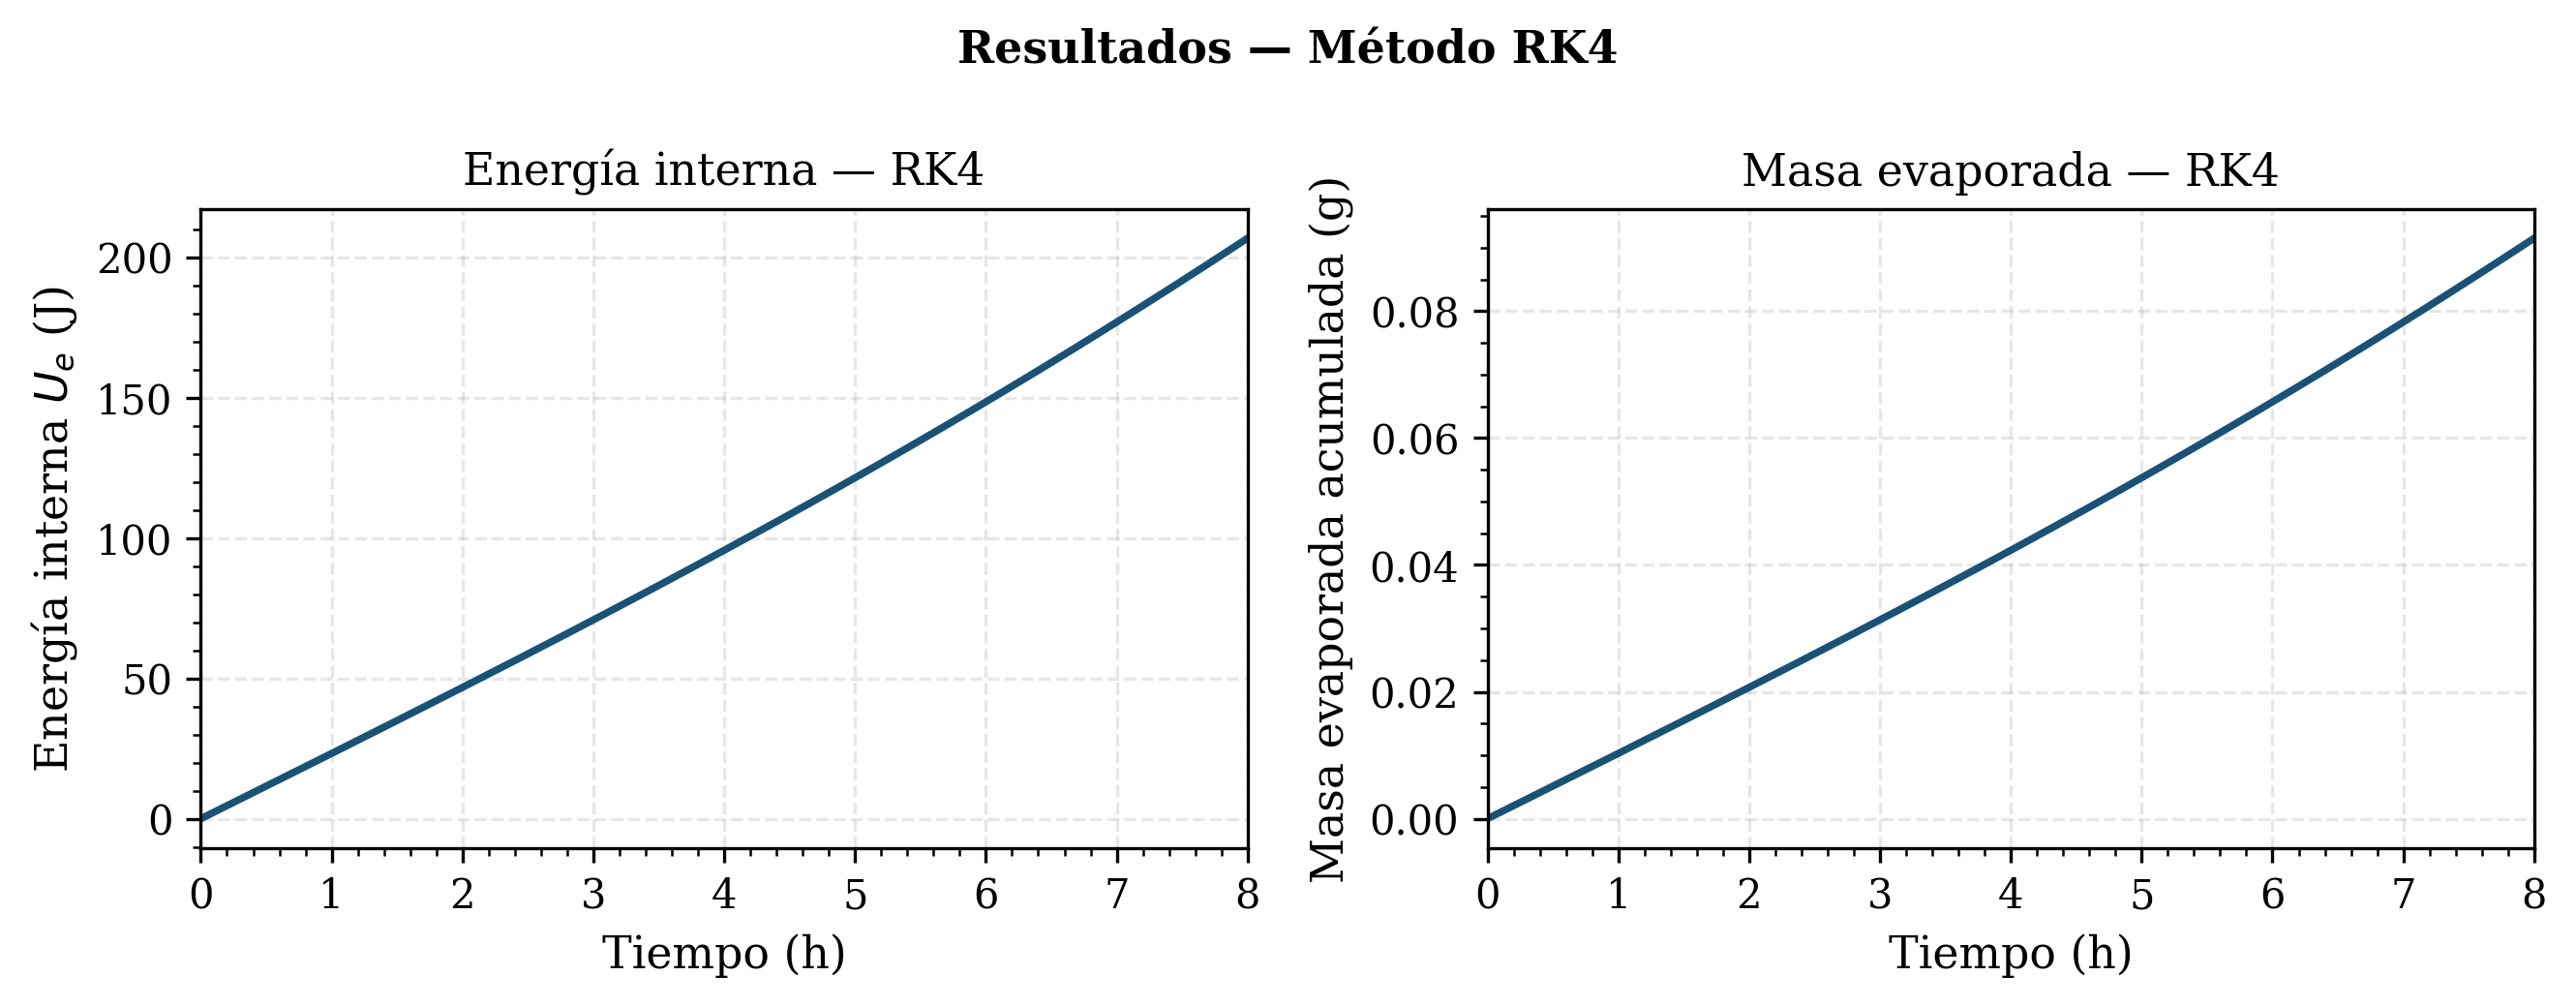
\includegraphics[width=0.48\textwidth]{comparacion_rk4.png}
\caption{Energía interna y masa evaporada calculadas con el método RK4.}
\label{fig:rk4_detalles}
\end{figure}

\begin{figure}[H]
\centering
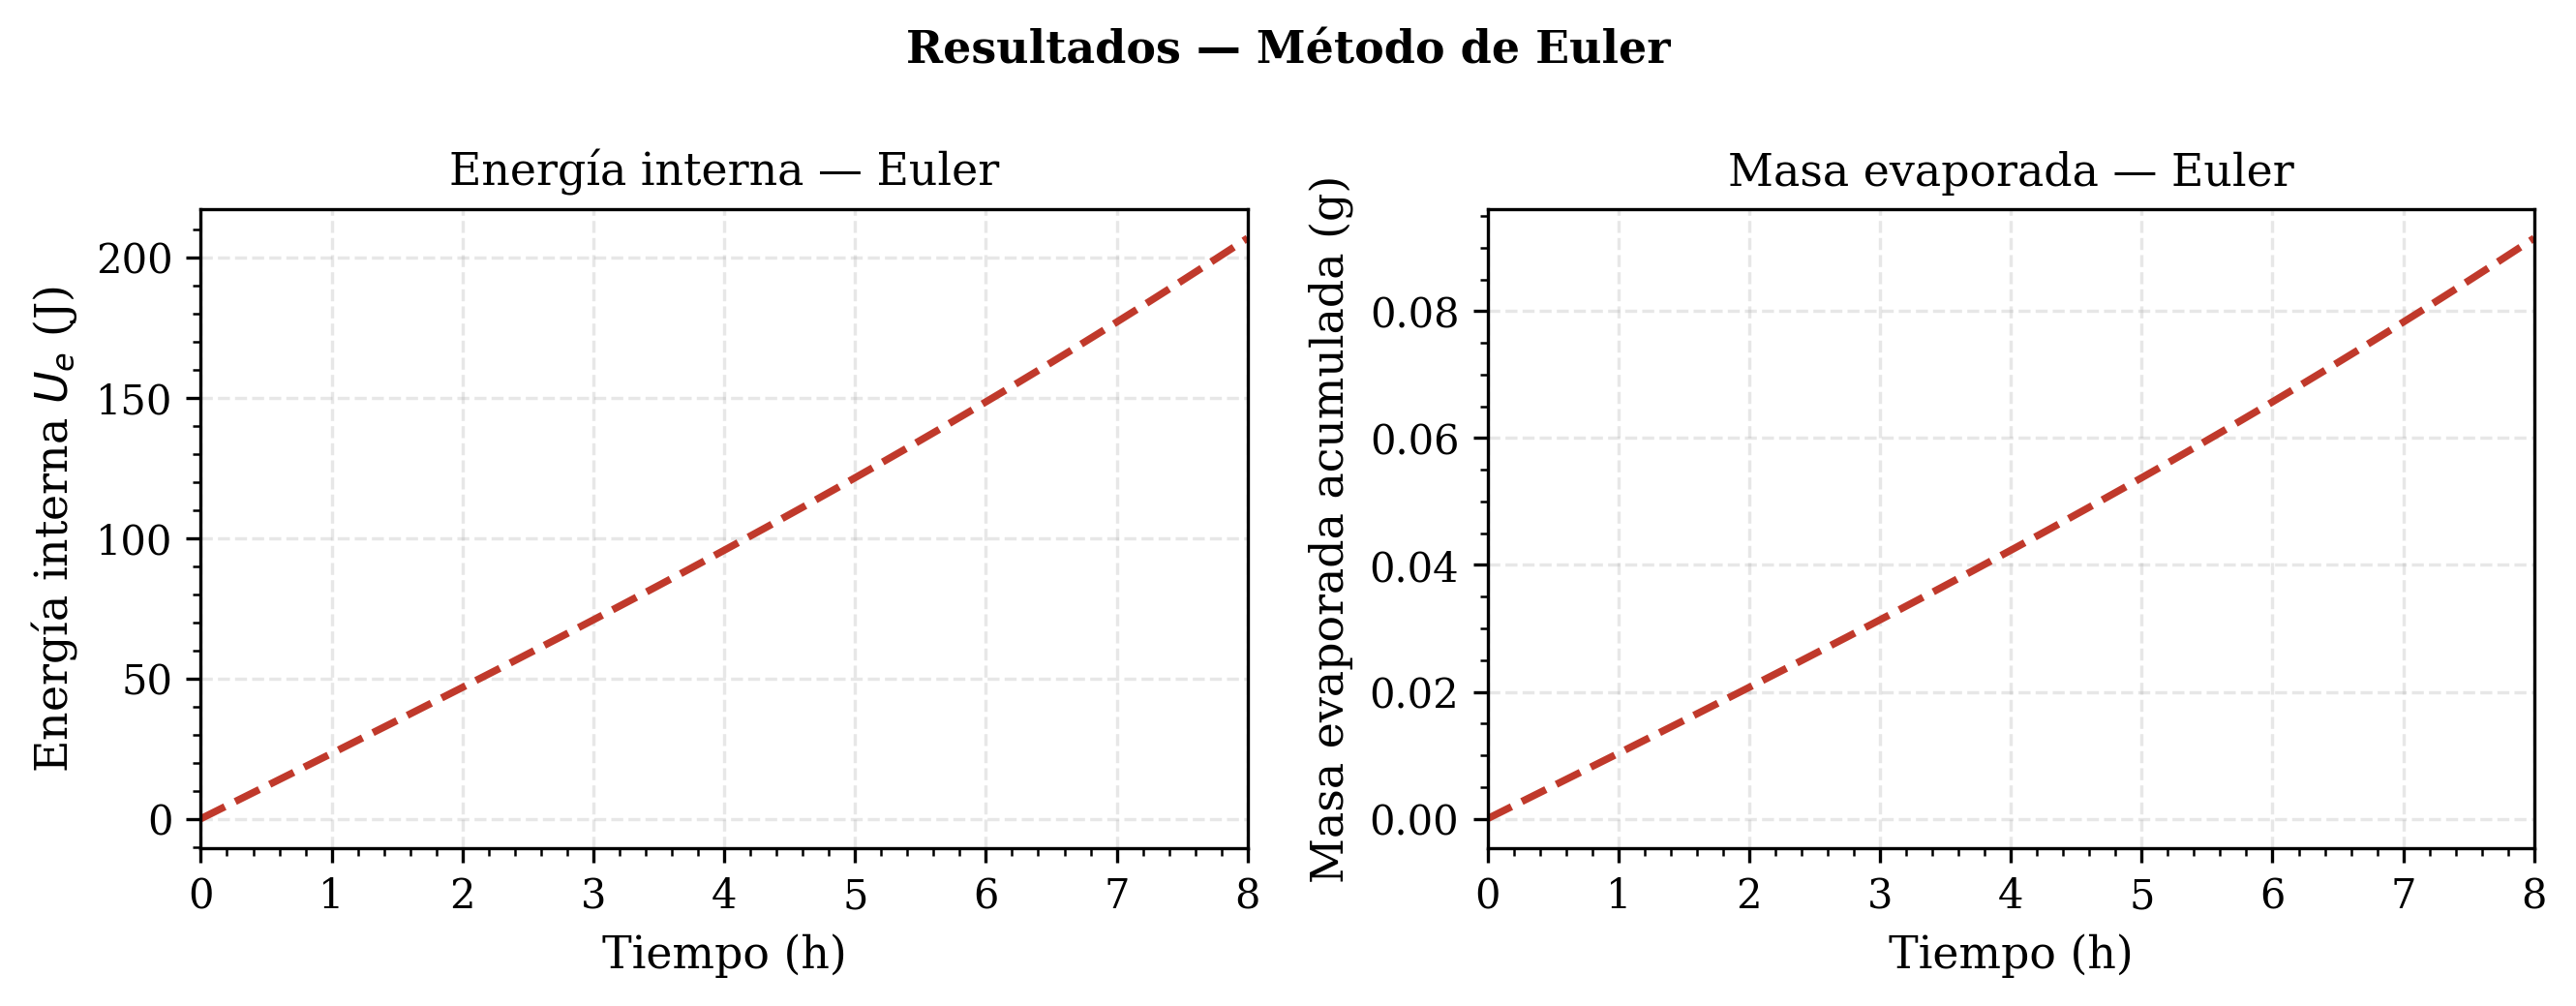
\includegraphics[width=0.48\textwidth]{comparacion_euler.png}
\caption{Energía interna y masa evaporada calculadas con el método de Euler.}
\label{fig:euler_detalles}
\end{figure}

El método RK4 presentó soluciones más suaves y estables en comparación con Euler, evidenciando menor acumulación de error numérico durante tiempos largos de integración.

\subsection{Estabilidad Numérica}

El método RK4 mostró estabilidad numérica durante todo el proceso de simulación, sin divergencias ni oscilaciones artificiales observables.

El uso de un paso temporal pequeño permitió mantener soluciones suaves y físicamente coherentes.

\subsection{Diseño Conceptual de la Marquesina}

Antes de presentar los resultados de la simulación, la Figura~\ref{fig:diseno_conceptual} muestra el diseño conceptual de la marquesina empleada como caso de estudio. La estructura consiste en un armazón de madera con techo a dos aguas de policarbonato translúcido y paredes laterales con malla de ventilación. En el interior se disponen \textbf{dos camas de secado elevadas} de $10\,\text{m} \times 1.60\,\text{m}$, soportadas por patas de madera a $0.80\,\text{m}$ del piso y separadas por un pasillo central de $0.60\,\text{m}$ para el volteo manual del café. Cada cama cuenta con un bastidor perimetral de madera, malla metálica en la base para favorecer la circulación de aire por debajo, y una capa de café de 4~cm de profundidad dividida en cinco capas horizontales que reciben el flujo de calor con atenuación exponencial. La sección A–A (Figura~\ref{fig:seccion_aa}) detalla la geometría de la cercha, las camas elevadas y el gradiente de factor de extinción entre capas.

\begin{figure}[H]
\centering
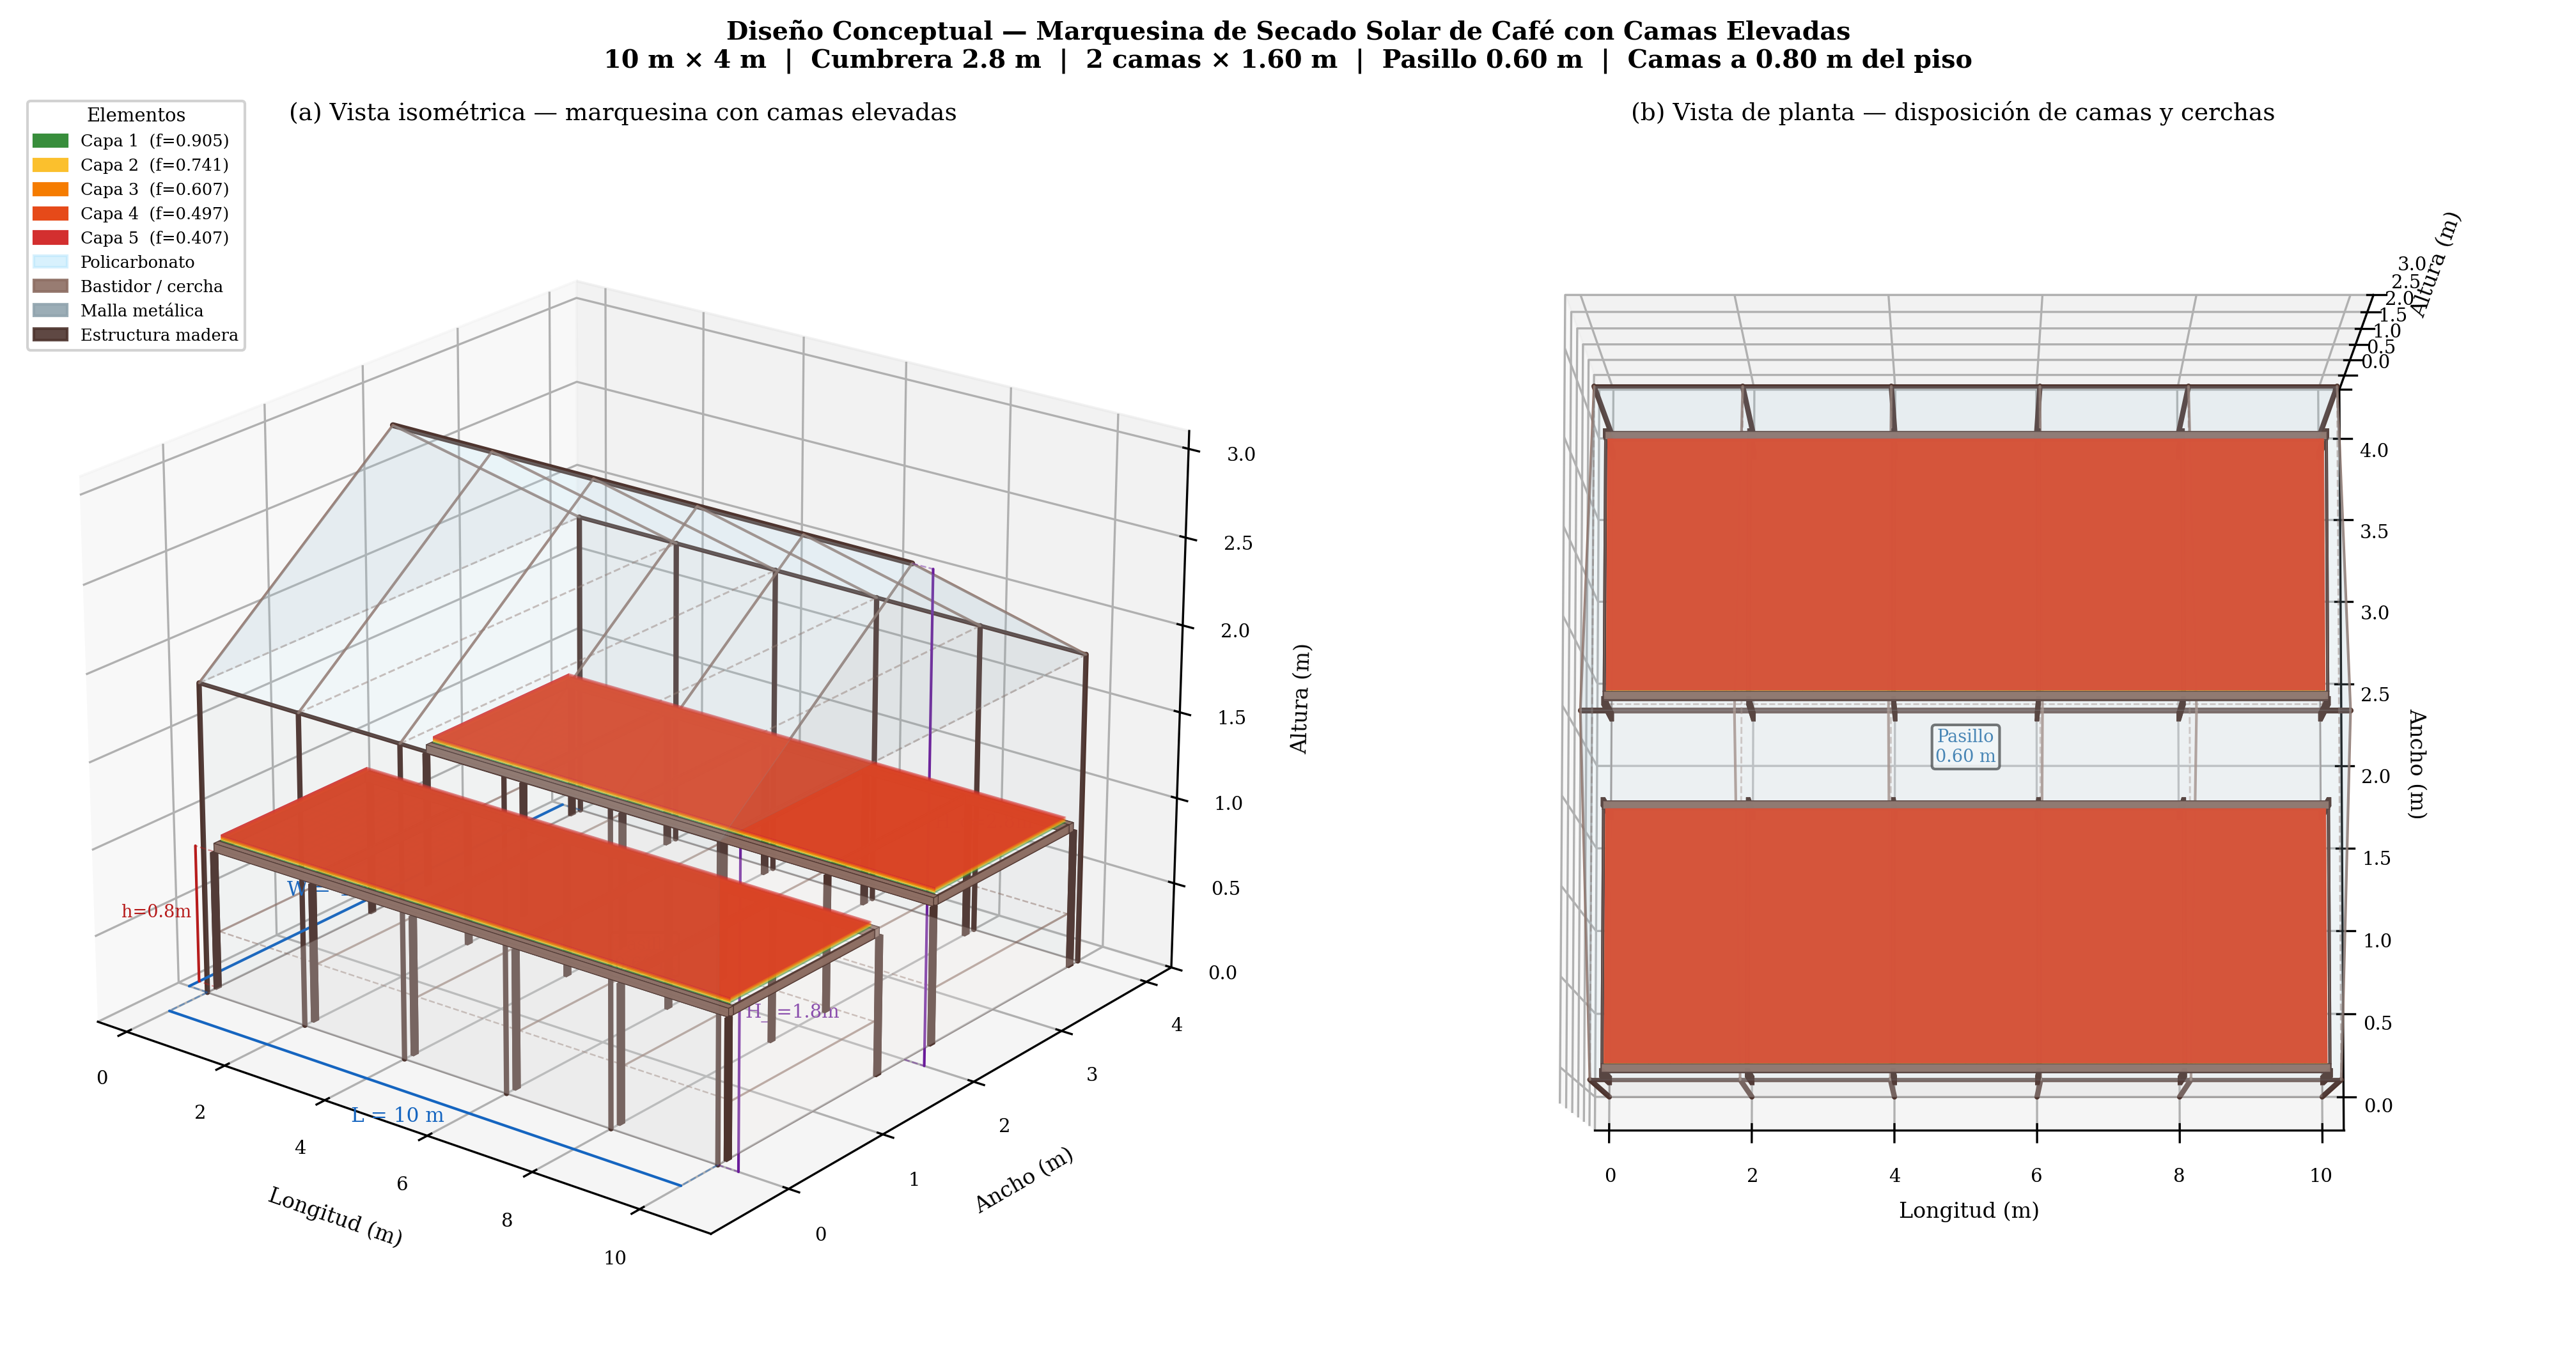
\includegraphics[width=0.48\textwidth]{marquesina_diseno_conceptual.png}
\caption{Diseño conceptual de la marquesina: vista isométrica con camas elevadas (izquierda) y planta (derecha). Se muestran las dos camas de $10\,\text{m}\times1.60\,\text{m}$, el pasillo central de $0.60\,\text{m}$ y las principales cotas estructurales.}
\label{fig:diseno_conceptual}
\end{figure}

\begin{figure}[H]
\centering
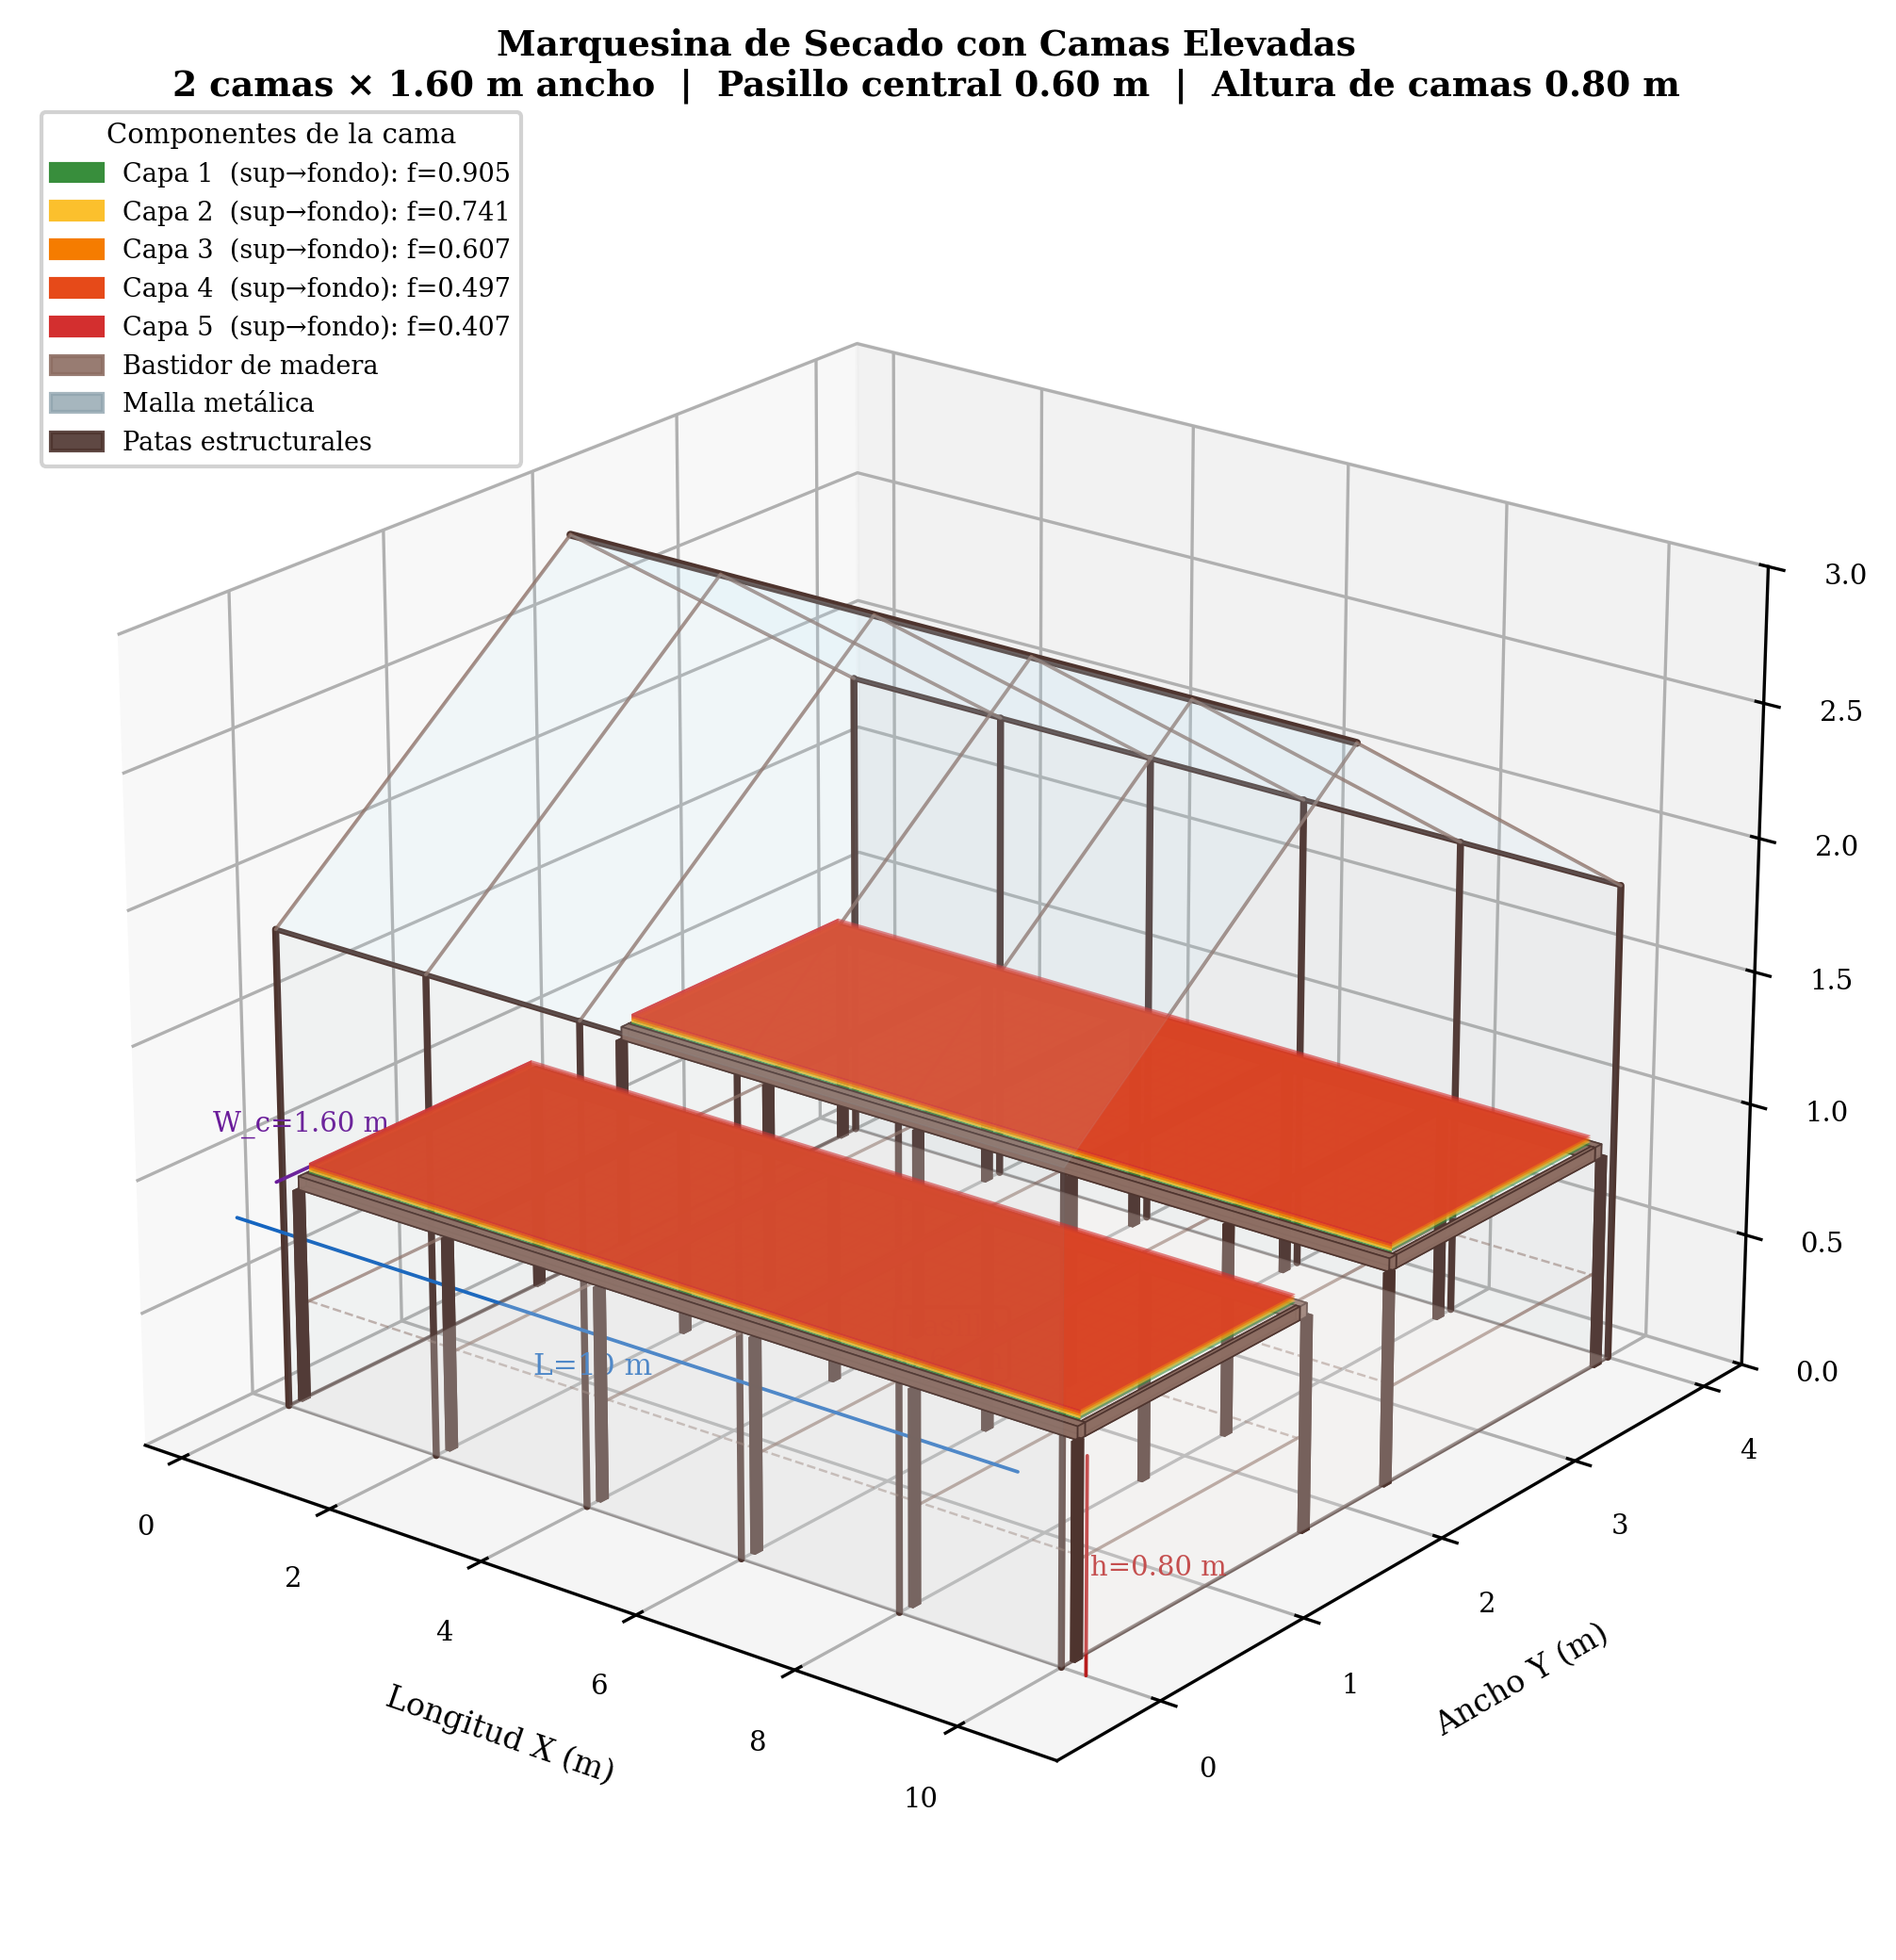
\includegraphics[width=0.48\textwidth]{camas_en_marquesina.png}
\caption{Vista 3D del ensamble completo: marquesina con camas de secado elevadas a $0.80\,\text{m}$, bastidor de madera, malla metálica y capa de café de 4~cm (cinco capas). Los colores de la sección frontal indican el gradiente de extinción del flujo de calor.}
\label{fig:camas_ensamble}
\end{figure}

\begin{figure}[H]
\centering
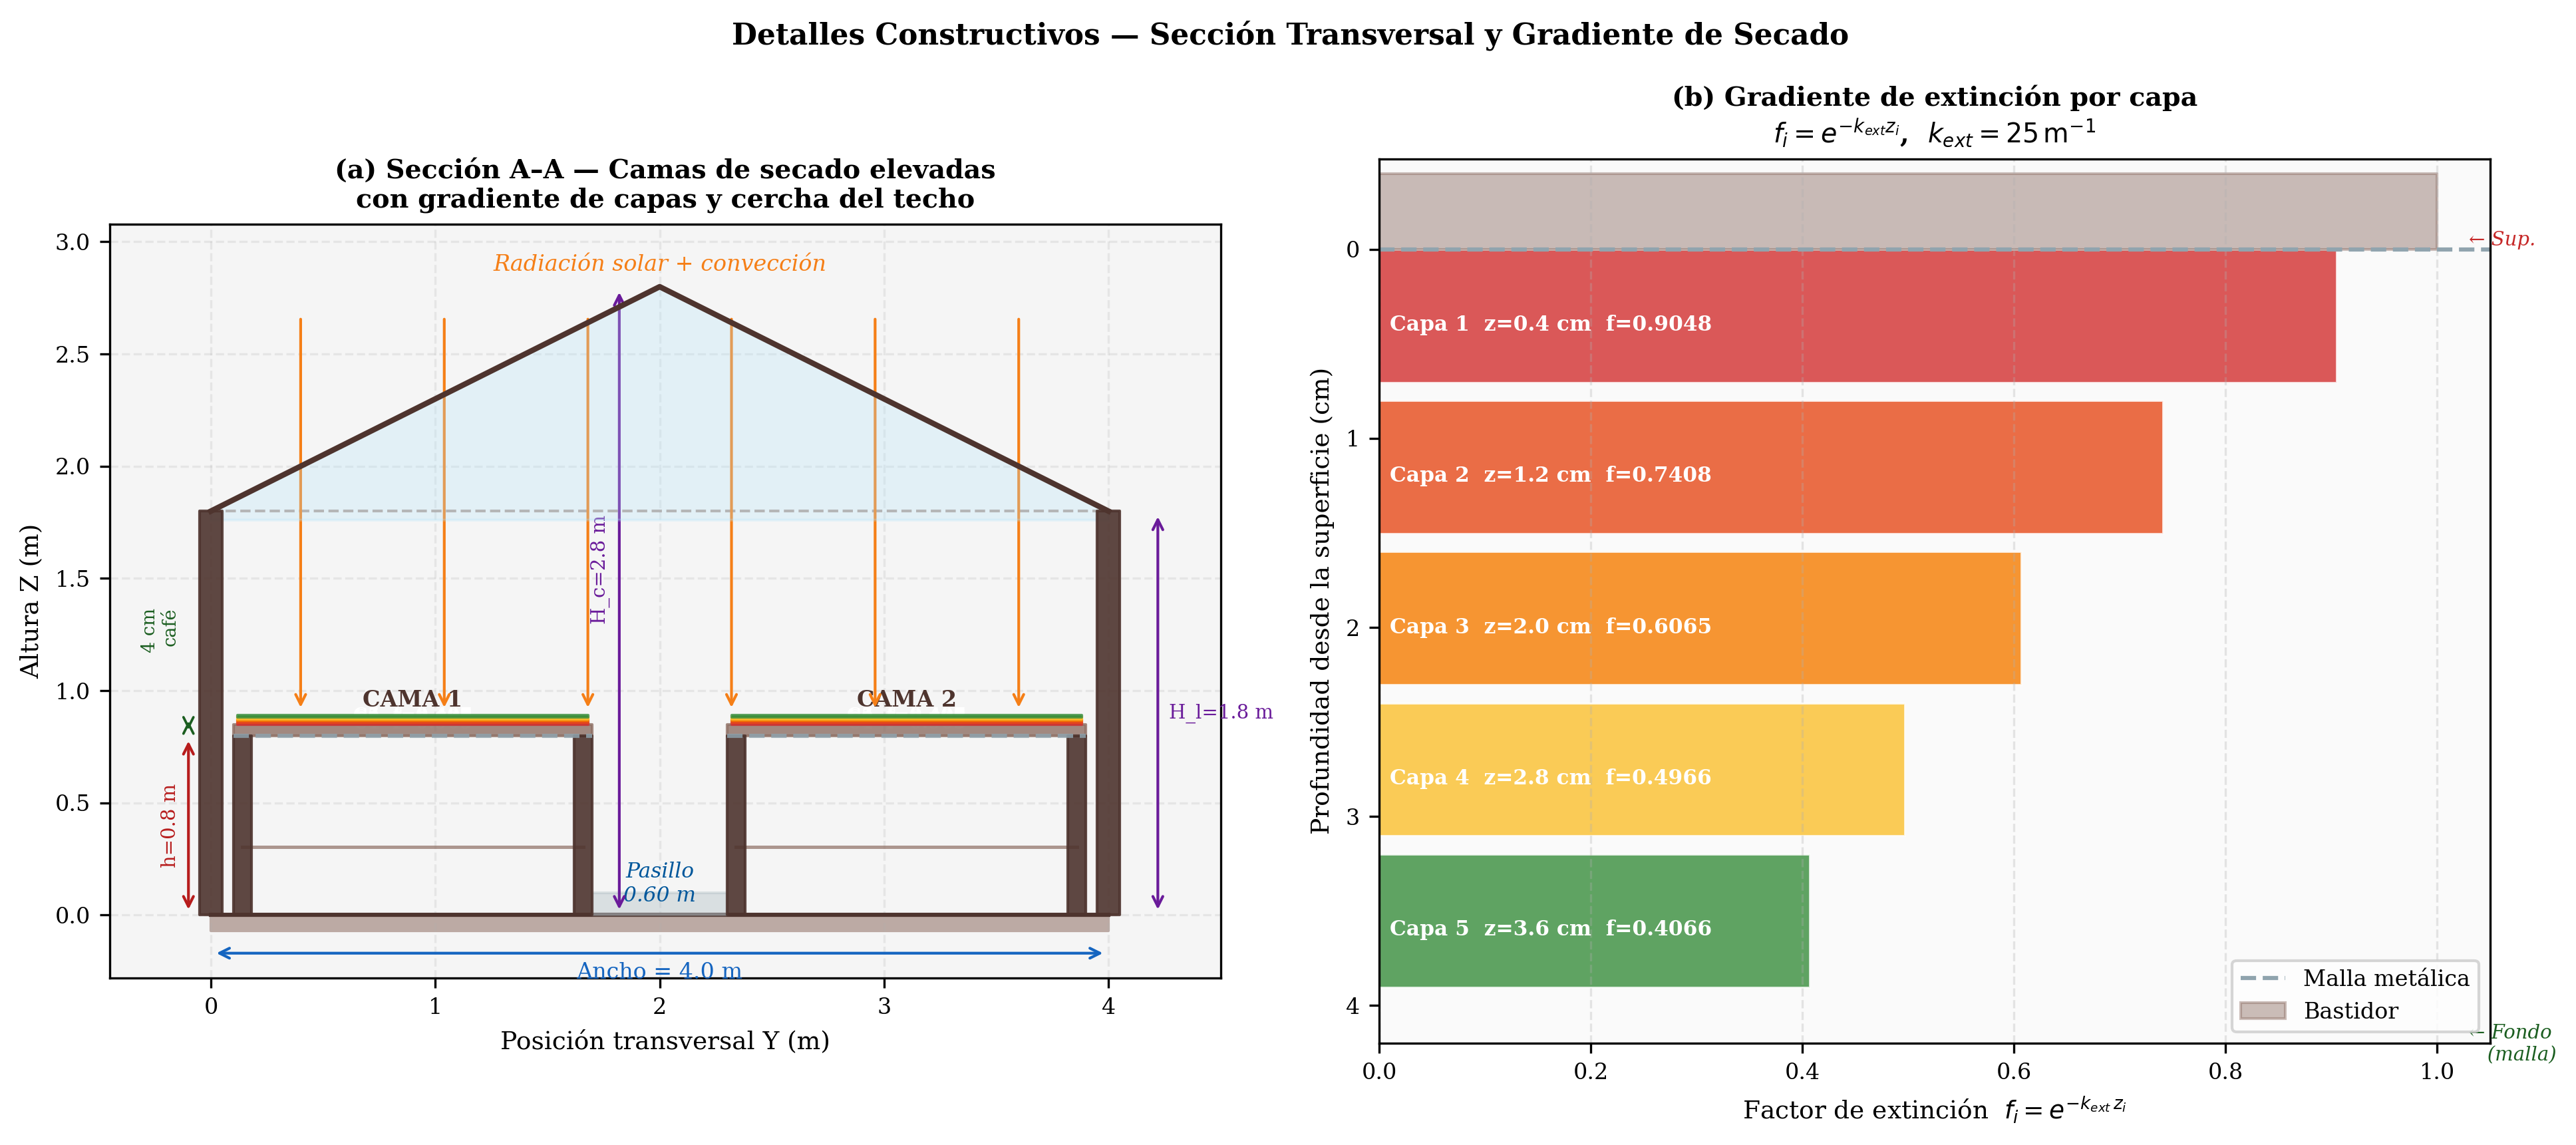
\includegraphics[width=0.48\textwidth]{marquesina_detalle_seccion.png}
\caption{(a) Sección transversal A–A: dos camas elevadas con sus patas, bastidor, malla y capas de café. (b) Factor de extinción $f_i = e^{-k_{ext}z_i}$ por capa ($k_{ext} = 25\,\text{m}^{-1}$): la capa superficial recibe el 90.5\% del flujo disponible mientras la del fondo recibe el 40.7\%.}
\label{fig:seccion_aa}
\end{figure}

\begin{figure}[H]
\centering
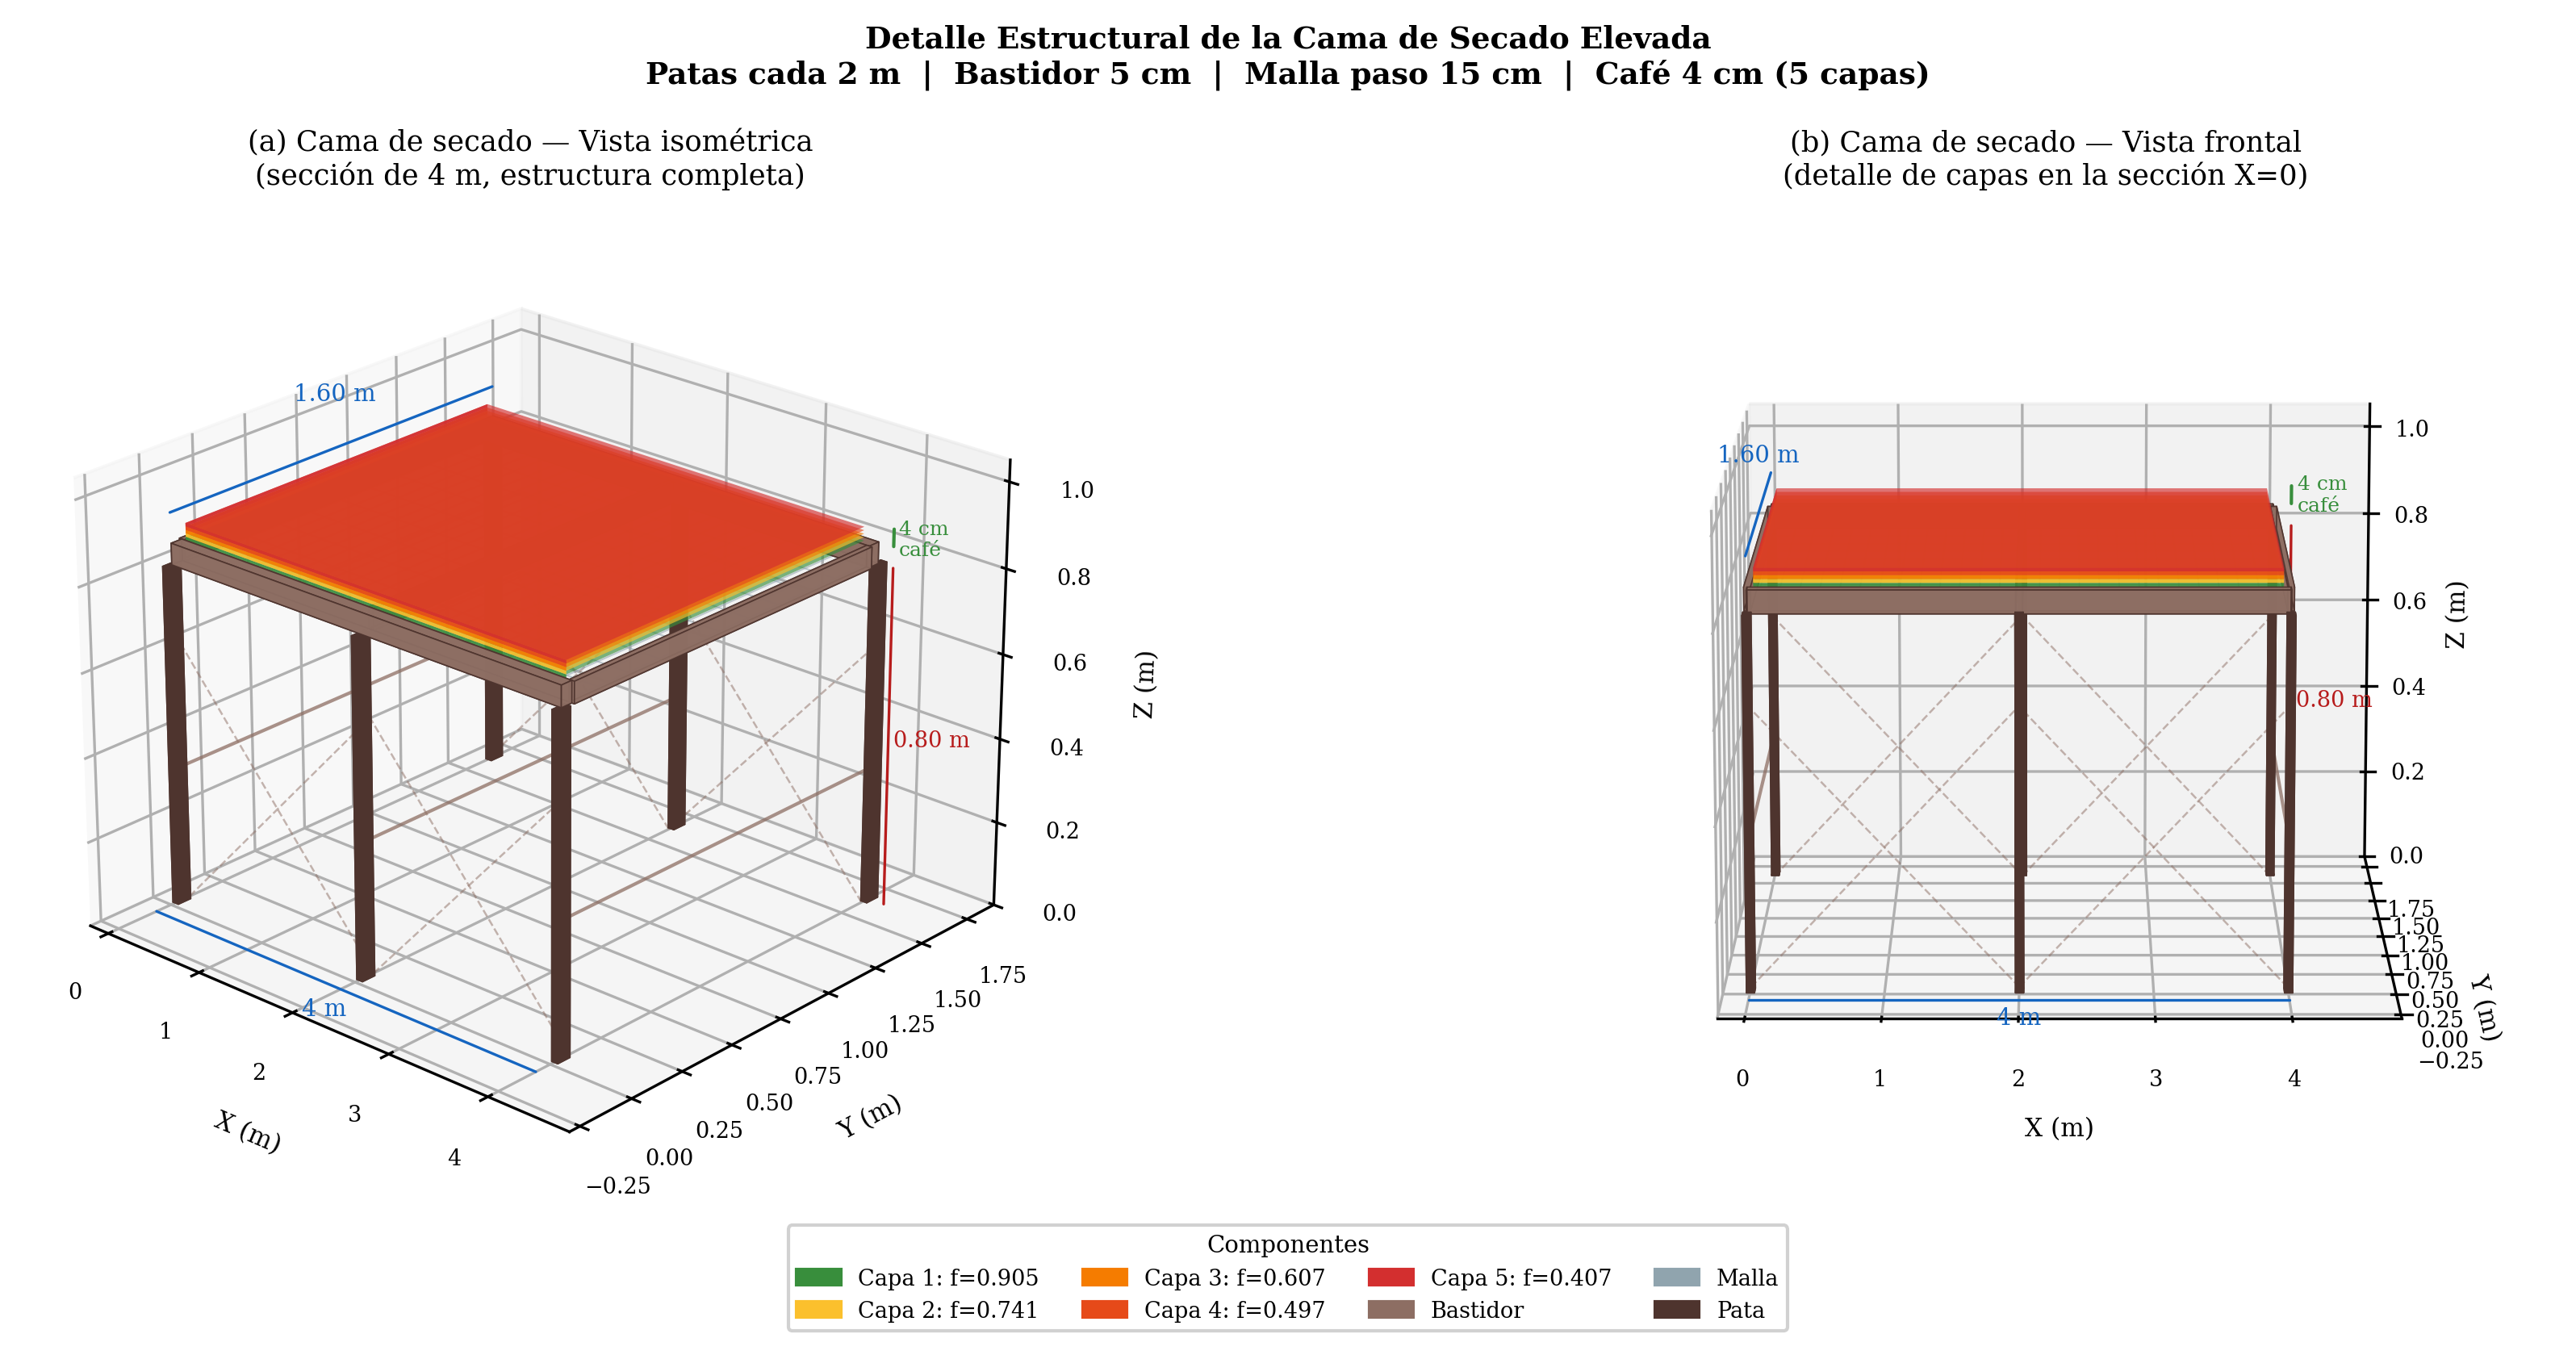
\includegraphics[width=0.48\textwidth]{camas_detalle_estructural.png}
\caption{Detalle estructural de una cama de secado: (a) vista isométrica con patas, riostras, bastidor, malla metálica y capas de café; (b) vista frontal con cotas de altura, ancho y espesor de la capa de café.}
\label{fig:camas_detalle}
\end{figure}

\begin{table}[H]
\centering
\caption{Parámetros de las camas de secado elevadas}
\begin{tabular}{llll}
\toprule
Parámetro & Símbolo & Valor & Unidad \\
\midrule
N$^\circ$ de camas & — & 2 & — \\
Longitud de cada cama & $L_c$ & 10 & m \\
Ancho de cada cama & $W_c$ & 1.60 & m \\
Área útil total & $A_u$ & 32 & m$^2$ \\
Pasillo central & — & 0.60 & m \\
Altura de patas & $h_p$ & 0.80 & m \\
Espesor del bastidor & — & 5 & cm \\
Paso entre patas & — & 2 & m \\
Paso de la malla & — & 15 & cm \\
Profundidad de café & $p_c$ & 4 & cm \\
N$^\circ$ de capas & $N_c$ & 5 & — \\
\bottomrule
\end{tabular}
\end{table}

\subsection{Simulación de la Marquesina Completa}

El modelo por capas se aplicó a una marquesina de 10~m~$\times$~4~m con aproximadamente $N = 2\,440\,966$ granos. La Figura~\ref{fig:marquesina_3d} muestra la representación tridimensional de la estructura y la distribución espacial de la humedad de los granos a las 4~horas de simulación. Los granos en las capas superiores (mayor exposición al flujo de calor) presentan colores hacia el rojo, indicando mayor pérdida de humedad, mientras que los granos del fondo conservan mayor contenido de agua.

\begin{figure}[H]
\centering
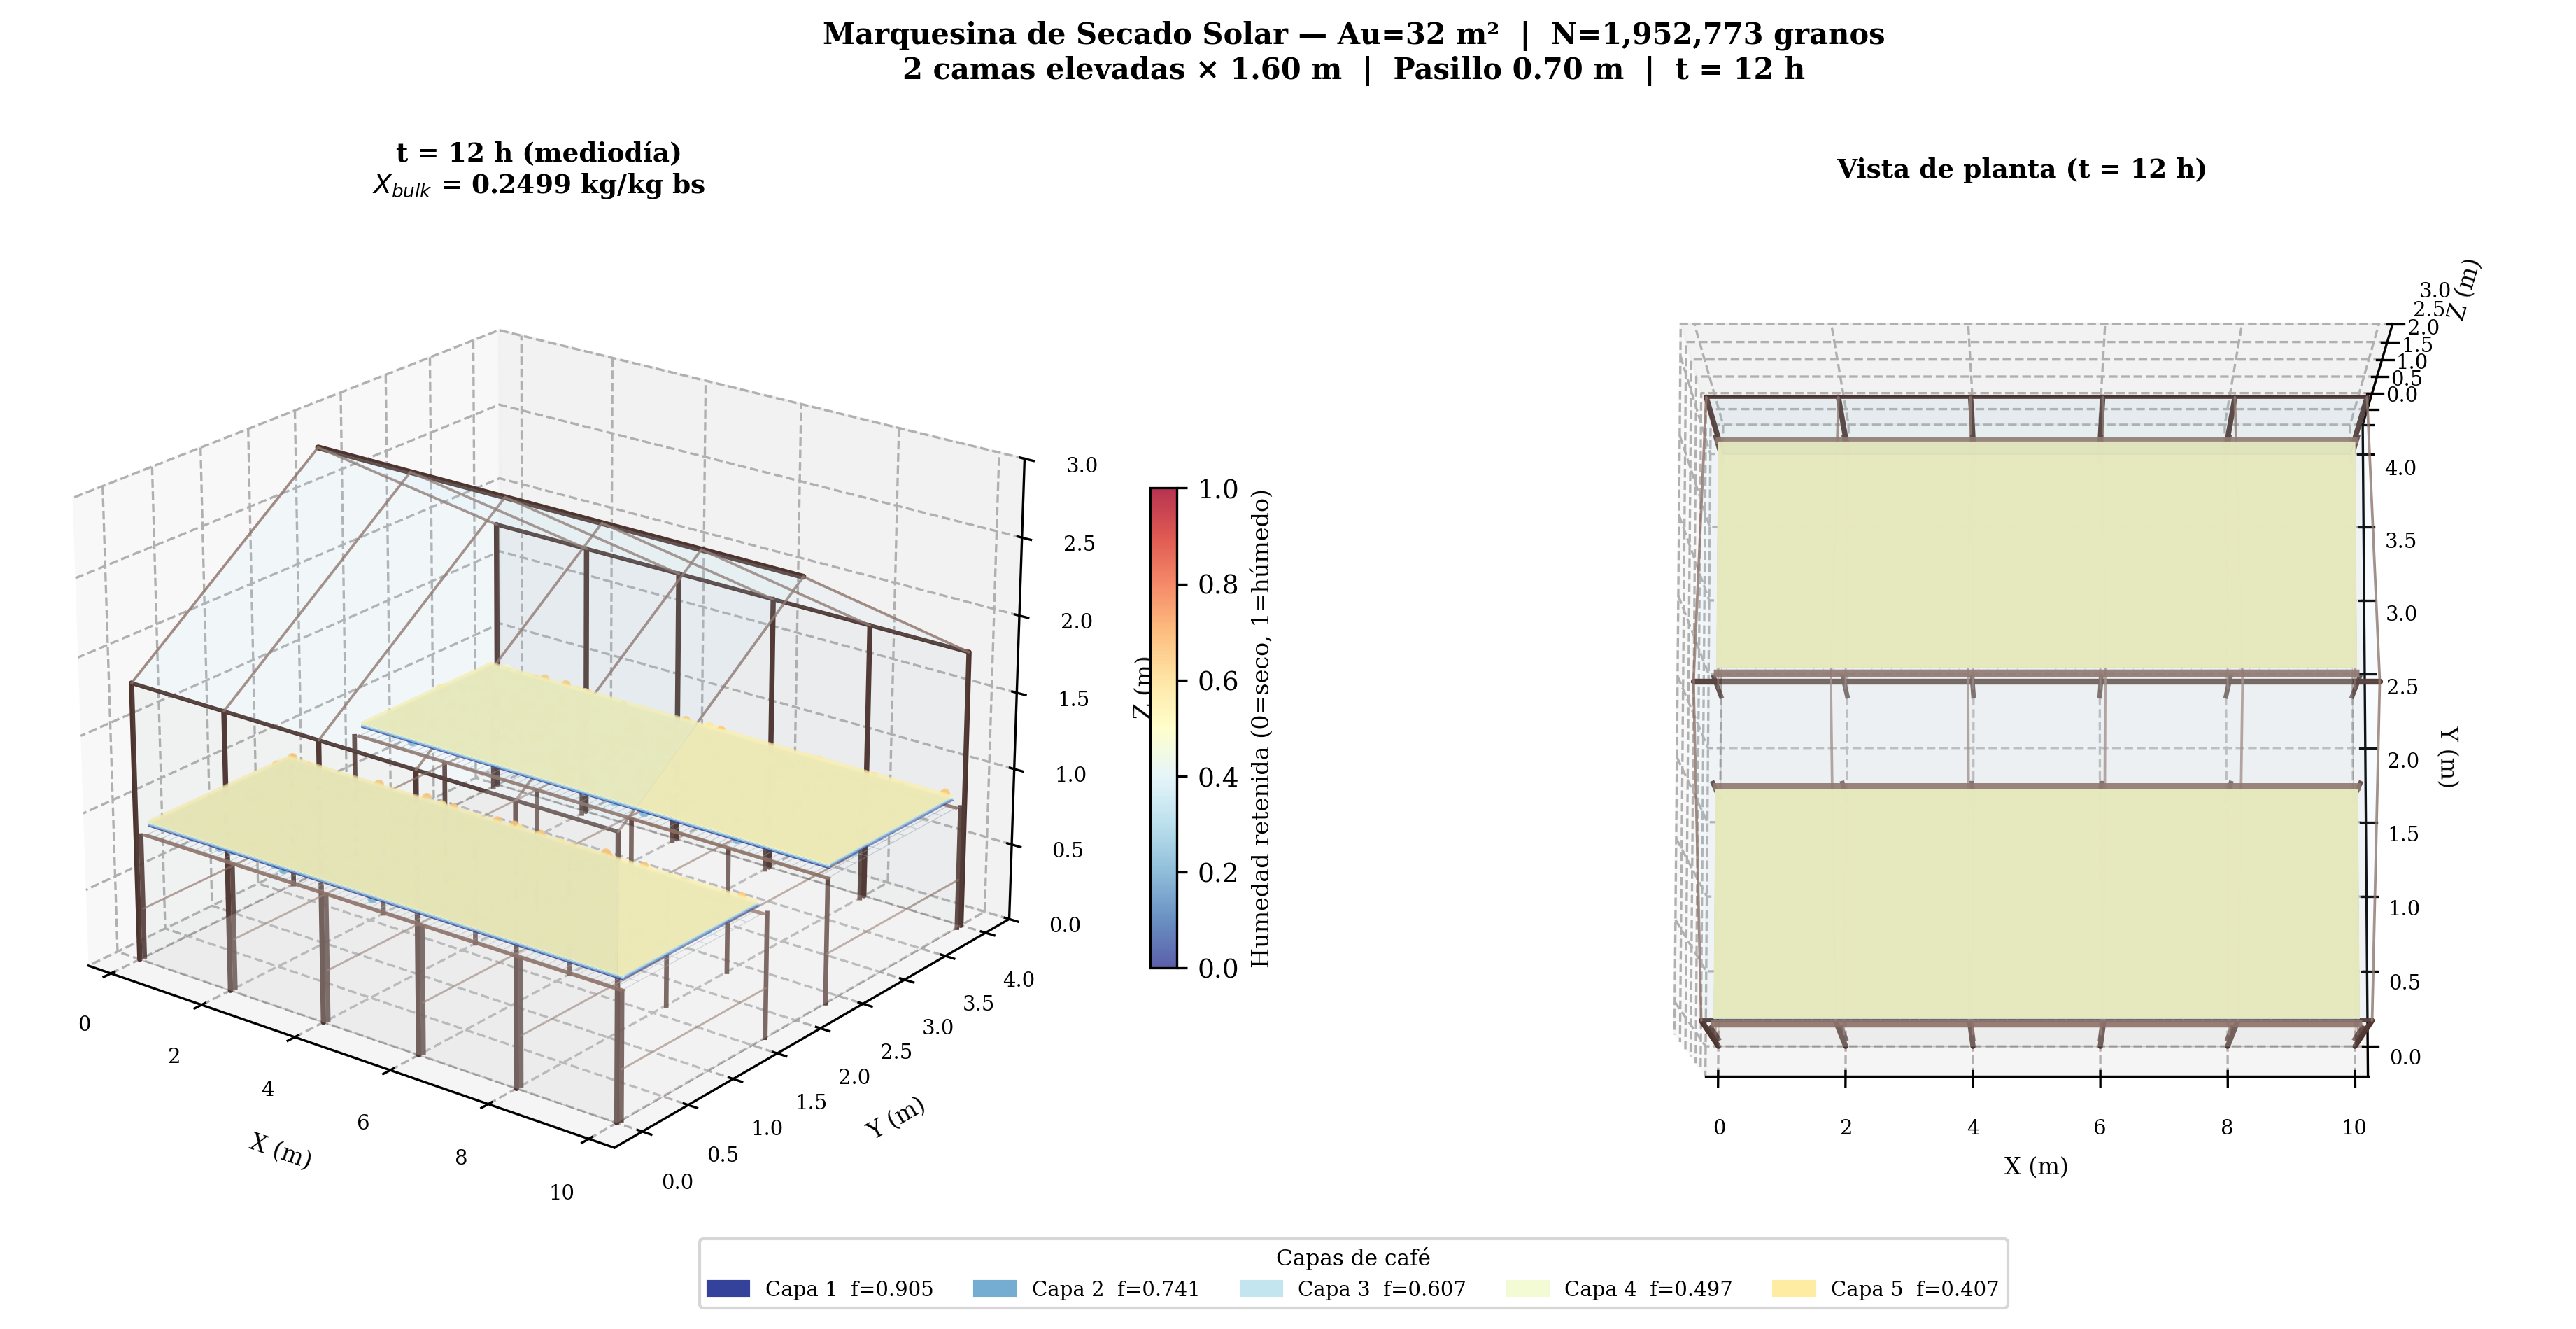
\includegraphics[width=0.48\textwidth]{marquesina_3d.png}
\caption{Modelo 3D de la marquesina a $t = 4\,\text{h}$. El color de cada grano indica la fracción de humedad retenida (azul~=~húmedo, rojo~=~seco). Escala vertical de la cama de café ampliada $\times 10$ para visualización.}
\label{fig:marquesina_3d}
\end{figure}

La Figura~\ref{fig:marquesina_metricas} presenta las métricas globales del proceso. El panel~(a) muestra la evolución de la humedad promedio del lote $X_{bulk}(t)$; los paneles (b) y (c) evidencian la masa de agua removida y el efecto diferencial del factor de extinción entre capas; el panel~(d) reproduce la temperatura ambiente utilizada como entrada.

\begin{figure}[H]
\centering
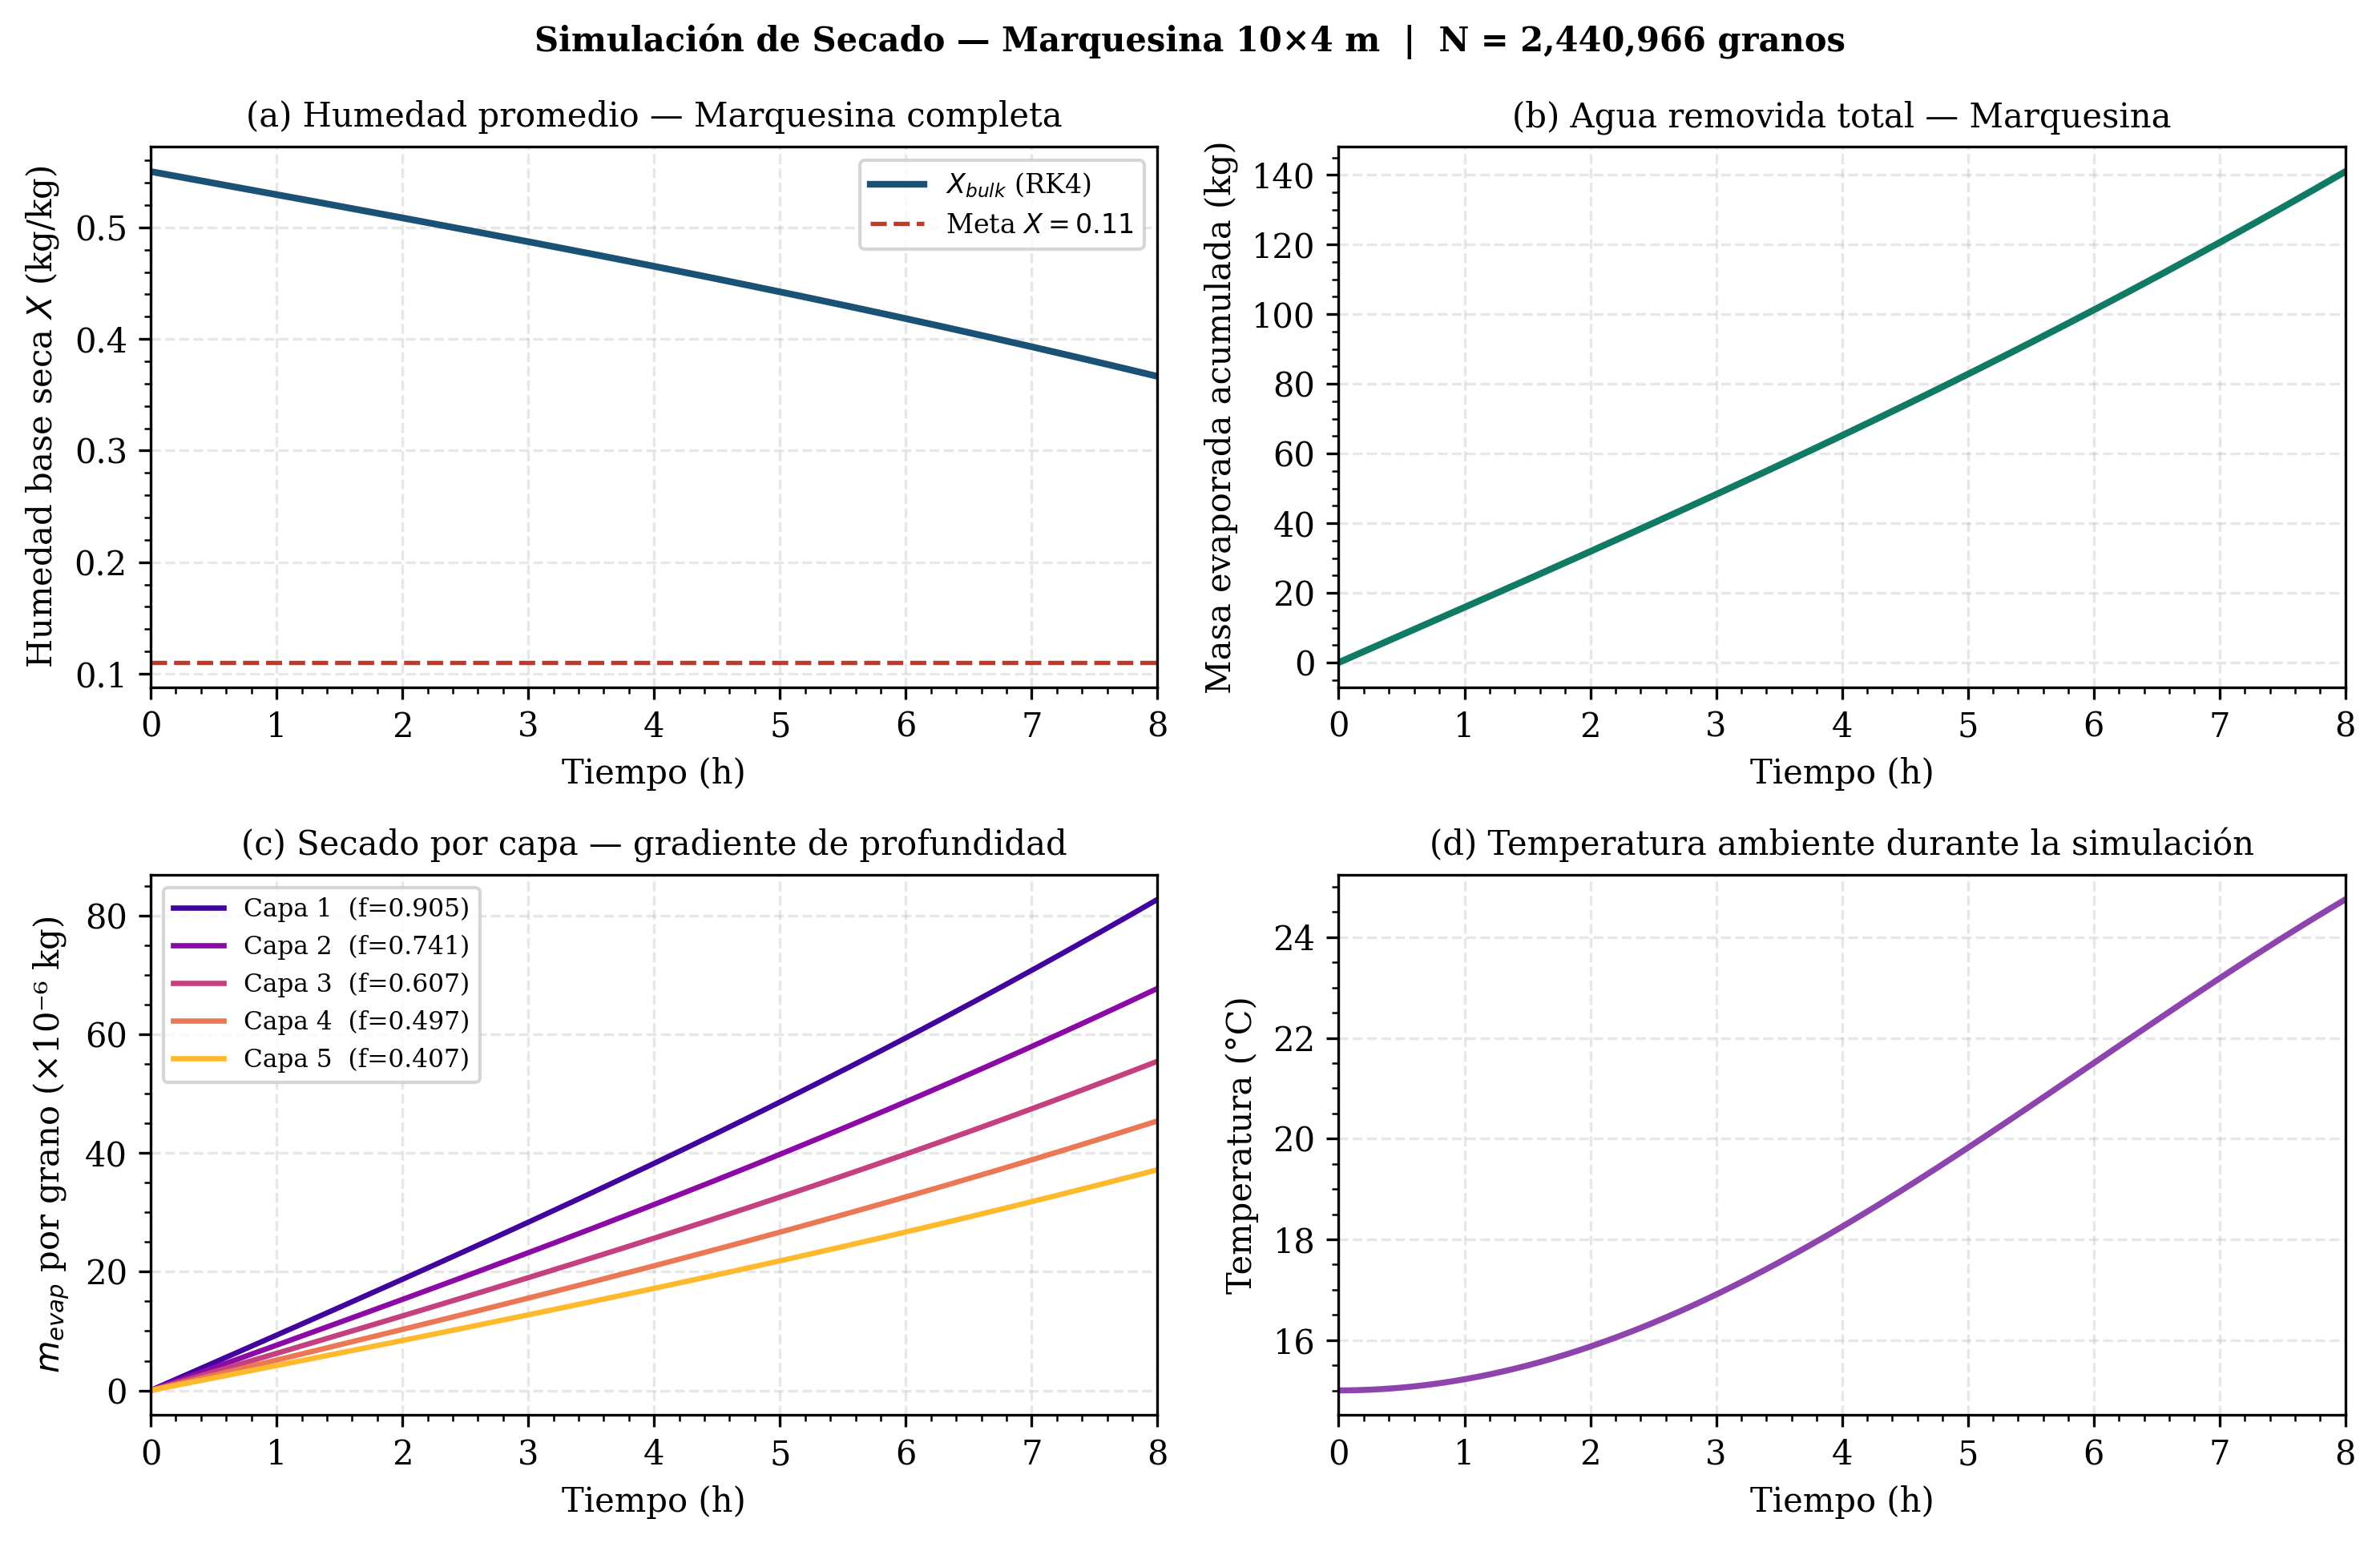
\includegraphics[width=0.48\textwidth]{marquesina_metricas.png}
\caption{Métricas globales de la marquesina durante 8 horas de secado: (a)~humedad promedio bulk, (b)~masa total evaporada, (c)~secado diferencial por capa y (d)~temperatura ambiente.}
\label{fig:marquesina_metricas}
\end{figure}

La Figura~\ref{fig:marquesina_snapshots} presenta cinco instantáneas temporales que ilustran la evolución progresiva del secado en la marquesina. En cada instante se observa un gradiente de color que confirma que la superficie de la cama se seca más rápidamente que las capas internas, en coherencia con el modelo de extinción exponencial definido en la Ec.~(\ref{eq:factor_capa}).

\begin{figure}[H]
\centering
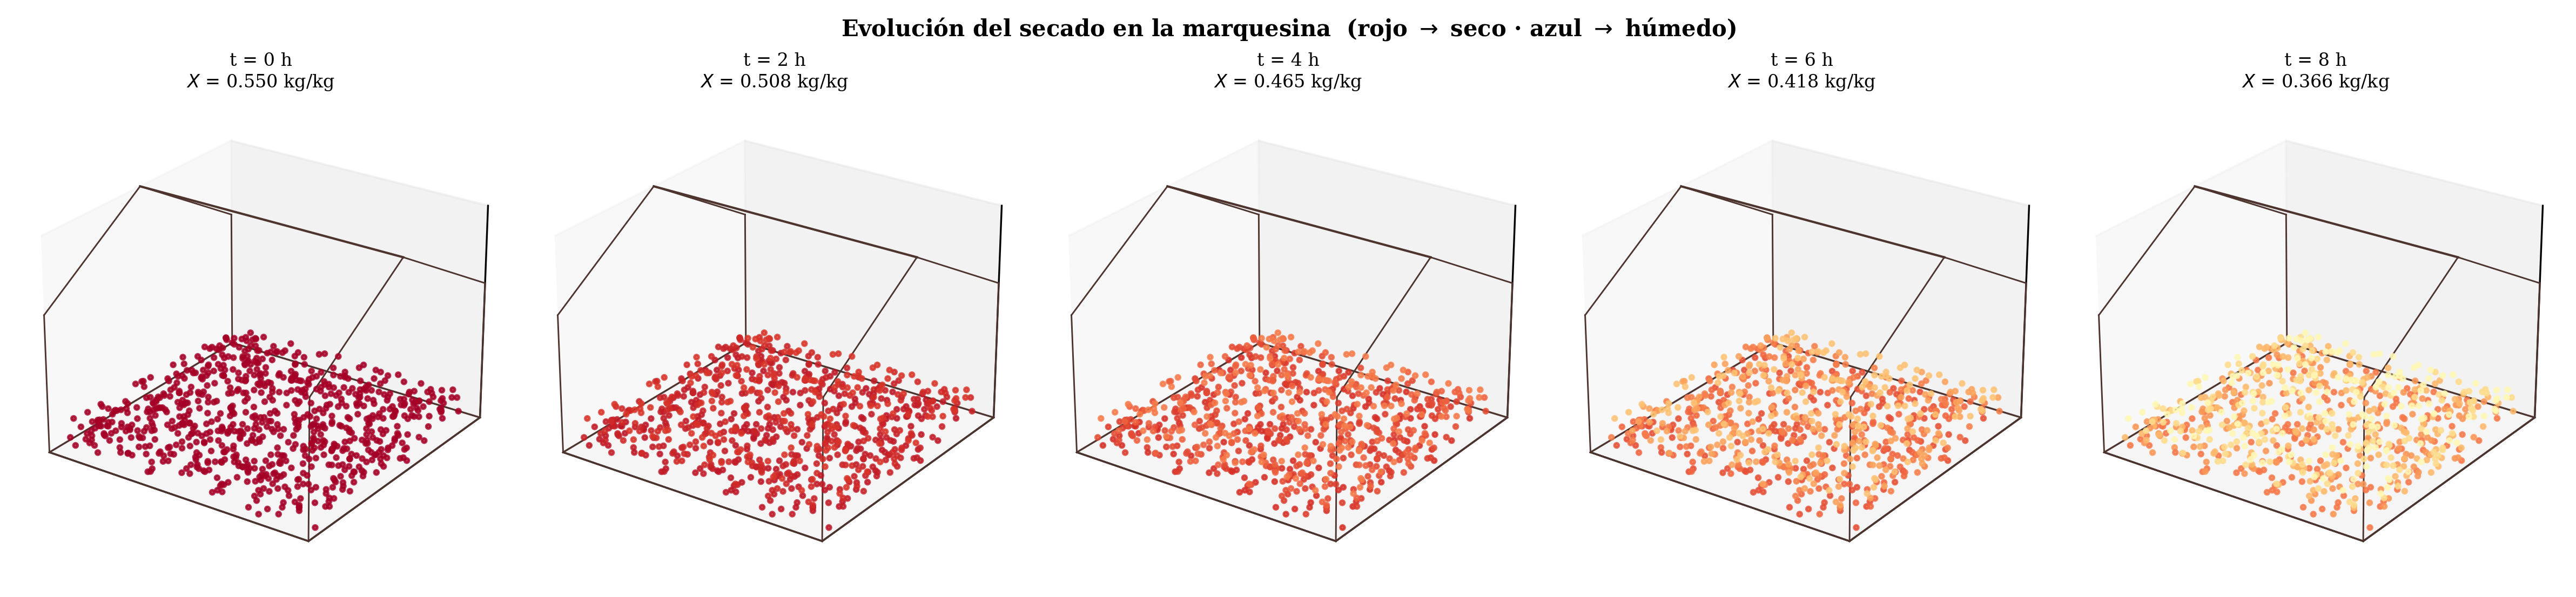
\includegraphics[width=0.48\textwidth]{marquesina_snapshots.png}
\caption{Evolución temporal del secado en la marquesina ($t = 0, 2, 4, 6, 8\,\text{h}$). Se indica el valor de $X_{bulk}$ en cada instante.}
\label{fig:marquesina_snapshots}
\end{figure}

\begin{table}[H]
\centering
\caption{Resultados de la simulación de la marquesina (8 horas)}
\begin{tabular}{lll}
\toprule
Variable & Valor & Unidad \\
\midrule
N$^\circ$ total de granos & 2\,440\,966 & — \\
Masa total húmeda inicial & 1\,190.40 & kg \\
Agua total inicial & 422.40 & kg \\
Agua evaporada acumulada (8~h) & 140.95 & kg \\
Porcentaje de agua removida & 33.37 & \% \\
Humedad inicial $X_0$ & 0.5500 & kg/kg (bs) \\
Humedad final $X(8\,\text{h})$ & 0.3665 & kg/kg (bs) \\
\bottomrule
\end{tabular}
\end{table}

Los resultados indican que, bajo las condiciones climáticas andinas modeladas, la marquesina remueve aproximadamente un tercio del agua inicial en 8~horas. Para alcanzar la humedad comercial objetivo ($X = 0.11\,\text{kg/kg}$) se requieren múltiples jornadas de secado, lo cual es consistente con los tiempos de 15 a 20 días reportados en la literatura para secado solar en Colombia~\cite{ref3}.

\subsection{Modelo PDE de Difusión — FlexPDE}

Como extensión del modelo de capas discretas, se plantea un modelo de difusión en derivadas parciales (EDP) que describe el campo continuo de humedad $W(z,t)$ en la cama de café. La ecuación gobernante y las condiciones de borde son:

\begin{equation}
\frac{\partial W}{\partial t} = D_{eff}\,\frac{\partial^2 W}{\partial z^2},
\quad z \in [0,\, p_c]
\label{eq:difusion}
\end{equation}

\begin{align}
\left.\frac{\partial W}{\partial z}\right|_{z=0} &= 0
\quad \text{(fondo impermeable)}
\label{eq:bc_fondo} \\[4pt]
-D_{eff}\left.\frac{\partial W}{\partial z}\right|_{z=p_c} &= h_m\,(W - W_{eq})
\quad \text{(evaporación superficial)}
\label{eq:bc_sup}
\end{align}

donde $D_{eff} = 5\times10^{-10}\,\text{m}^2/\text{s}$ es la difusividad efectiva de humedad en el lecho, $h_m = 10^{-7}\,\text{m/s}$ el coeficiente de transferencia de masa y $W_{eq} = 0.12\,\text{kg/kg}$ la humedad de equilibrio. El número de Biot másico $Bi_m = h_m\,p_c/D_{eff} = 8$ indica un régimen de control mixto entre resistencia superficial y difusión interna. El número de Fourier al finalizar la simulación,

\begin{equation}
Fo = \frac{D_{eff}\,t_{fin}}{p_c^2}
   = \frac{5\times10^{-10}\times 28800}{(0.04)^2}
   \approx 9\times10^{-3} \ll 1
\label{eq:fourier}
\end{equation}

confirma que el proceso difusivo es lento respecto a la escala de la cama: en 8 horas el frente de secado alcanza apenas $\delta \approx 2\sqrt{D_{eff}\,t} \approx 0.76\,\text{cm}$ desde la superficie, mientras el interior permanece sin perturbación significativa.

Este sistema fue resuelto numéricamente mediante el esquema Crank-Nicolson (CN) sobre una malla de 200 nodos con paso temporal $\Delta t = 60\,\text{s}$. El esquema CN requiere resolver en cada paso el sistema tridiagonal:

\begin{equation}
\mathbf{A}\,\mathbf{W}^{n+1} = \mathbf{b}(\mathbf{W}^n)
\label{eq:tridiag}
\end{equation}

resuelto eficientemente con el algoritmo de Thomas $\mathcal{O}(N)$. El script FlexPDE \texttt{secado\_cafe.pde} implementa esta misma formulación mediante elementos finitos adaptativos con malla de 60 nodos y tolerancia $\epsilon = 10^{-5}$.

\subsection{Resultados del Modelo PDE}

La Figura~\ref{fig:pde_mapa} muestra el mapa espacio-temporal de la humedad $W(z,t)$ y la evolución de la temperatura superficial quasi-estacionaria. El frente de secado avanza desde la superficie ($z = p_c = 4\,\text{cm}$) hacia el fondo, con una profundidad de penetración de $\delta \approx 2\sqrt{D_{eff}\,t} = 0.76\,\text{cm}$ a las 8 horas, coherente con el tiempo difusivo característico $\tau_D = p_c^2/D_{eff} \approx 889\,\text{h}$ y con el bajo número de Fourier calculado en la Ec.~(\ref{eq:fourier}).

\begin{figure}[H]
\centering
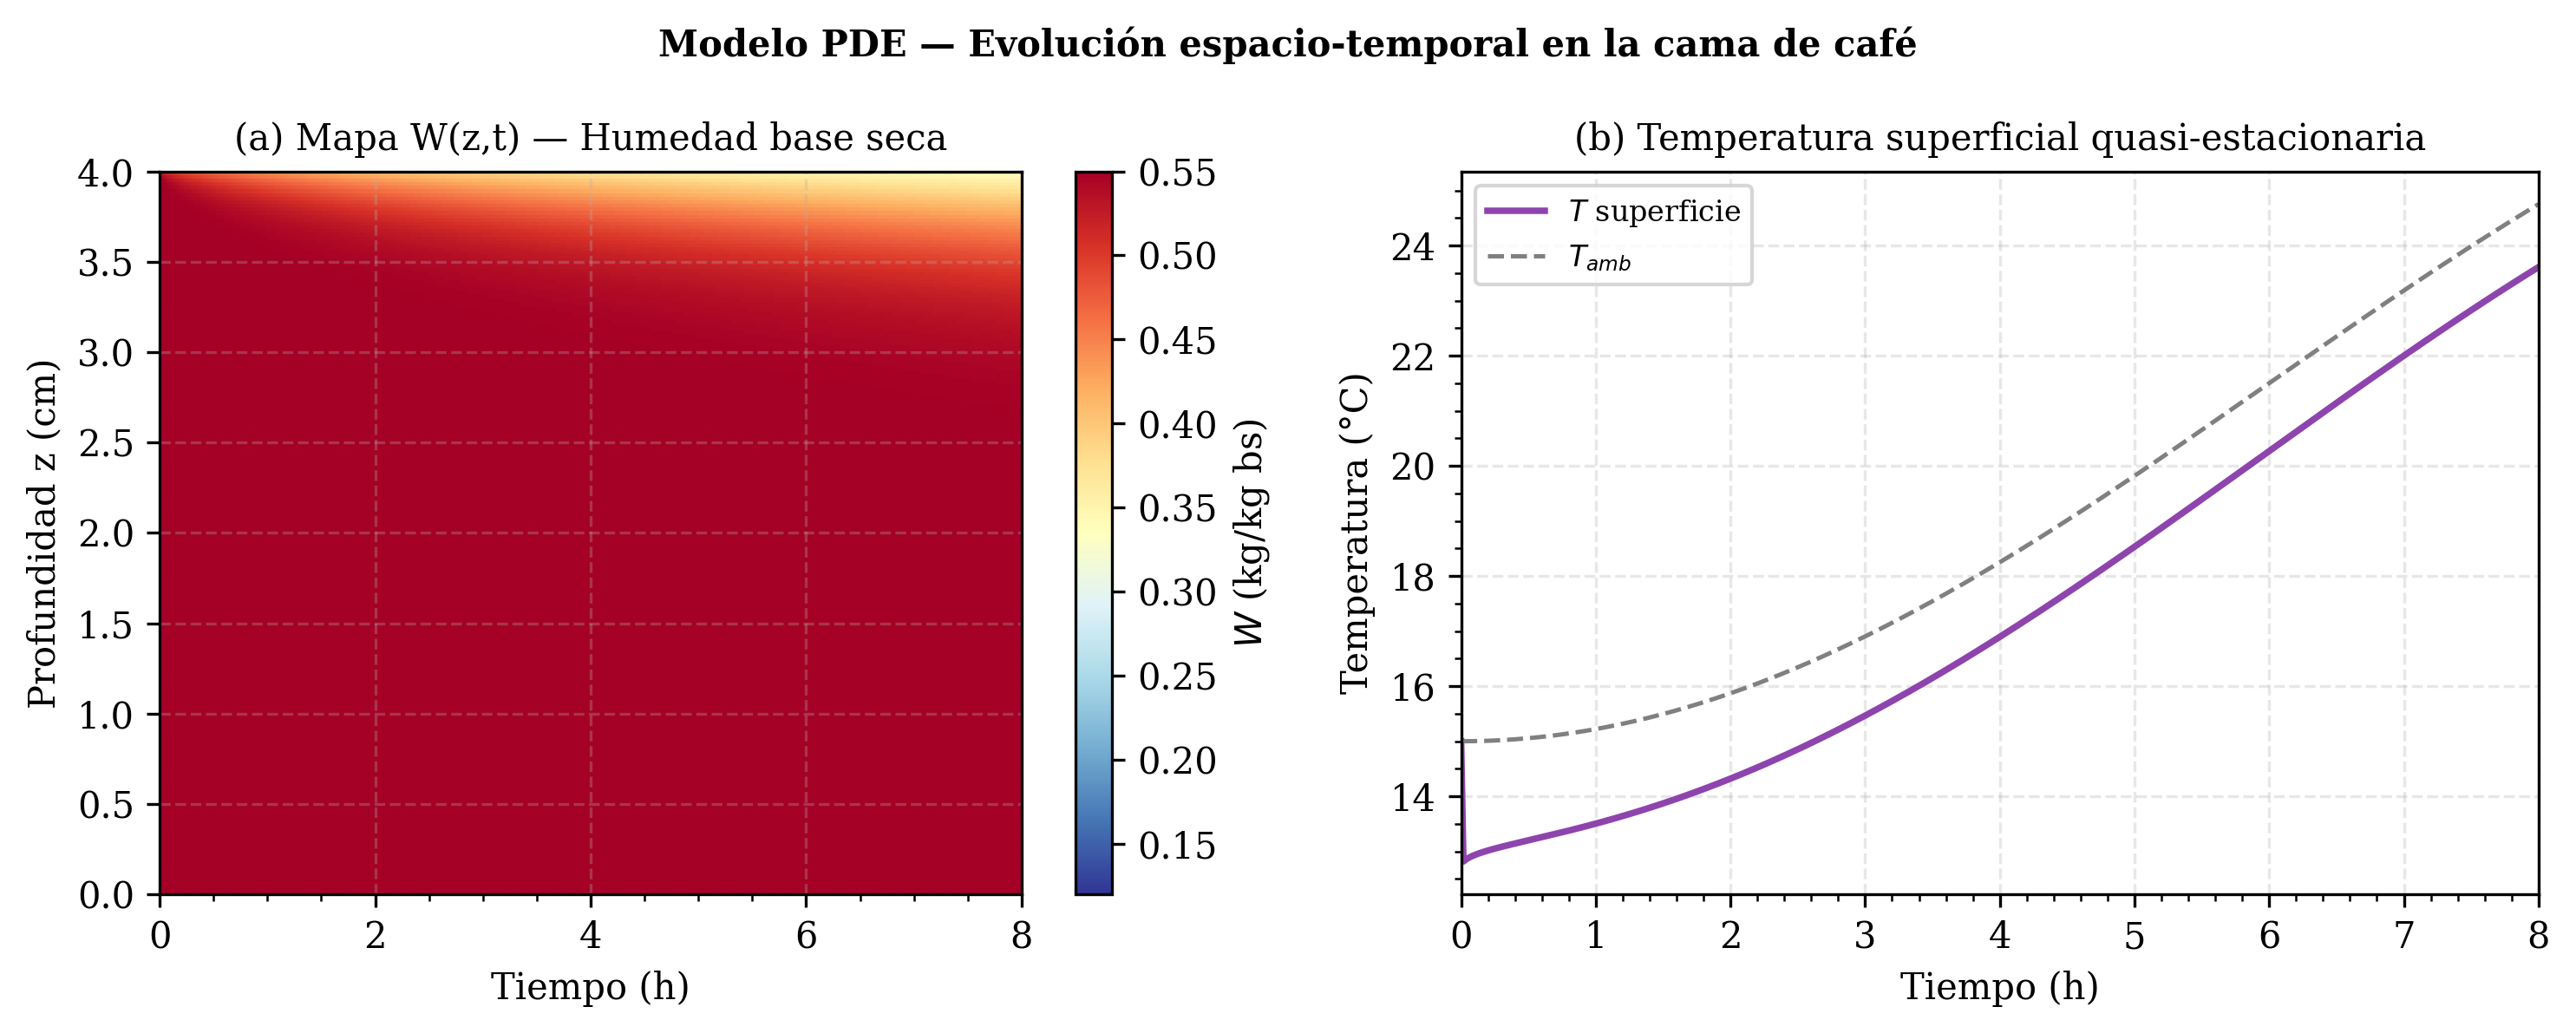
\includegraphics[width=0.48\textwidth]{pde_mapa_espacio_tiempo.png}
\caption{Mapa espacio-temporal $W(z,t)$ (izquierda) y temperatura superficial quasi-estacionaria (derecha). El color en el mapa indica la fracción de humedad retenida.}
\label{fig:pde_mapa}
\end{figure}

La Figura~\ref{fig:pde_perfiles} presenta los perfiles de humedad $W(z)$ a cinco instantes temporales. Se observa que el interior del lecho permanece sin modificación significativa durante las 8 horas de simulación, mientras que la zona cercana a la superficie experimenta una reducción progresiva de humedad.

\begin{figure}[H]
\centering
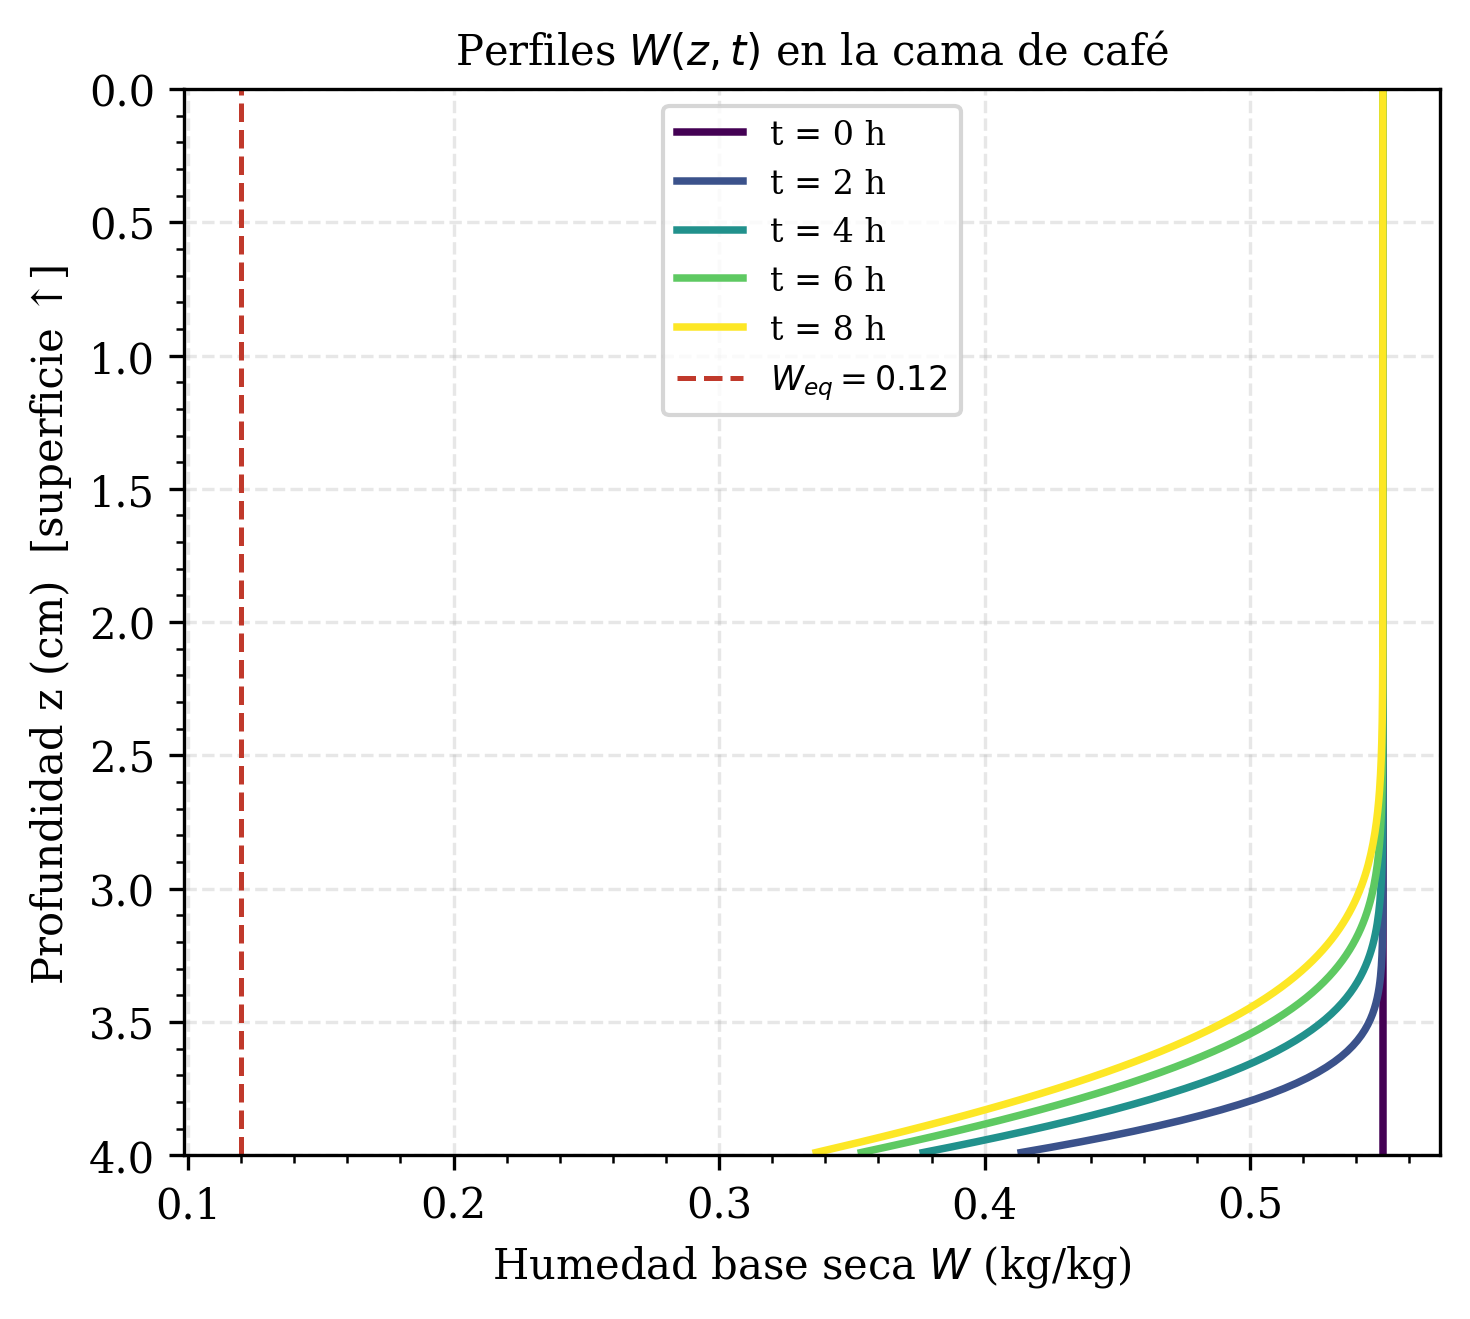
\includegraphics[width=0.40\textwidth]{pde_perfiles.png}
\caption{Perfiles de humedad $W(z)$ a $t = 0, 2, 4, 6, 8\,\text{h}$. La línea roja punteada indica la humedad de equilibrio $W_{eq} = 0.12\,\text{kg/kg}$.}
\label{fig:pde_perfiles}
\end{figure}

La Figura~\ref{fig:pde_comparacion} contrasta el perfil continuo del modelo PDE con los valores discretos del modelo ODE por capas. El modelo PDE resuelve el gradiente exacto, mientras que el modelo ODE representa cada capa con un valor promedio. Ambas formulaciones son consistentes en la tendencia general, con el modelo ODE ofreciendo mayor eficiencia computacional a expensas de resolución espacial.

\begin{figure}[H]
\centering
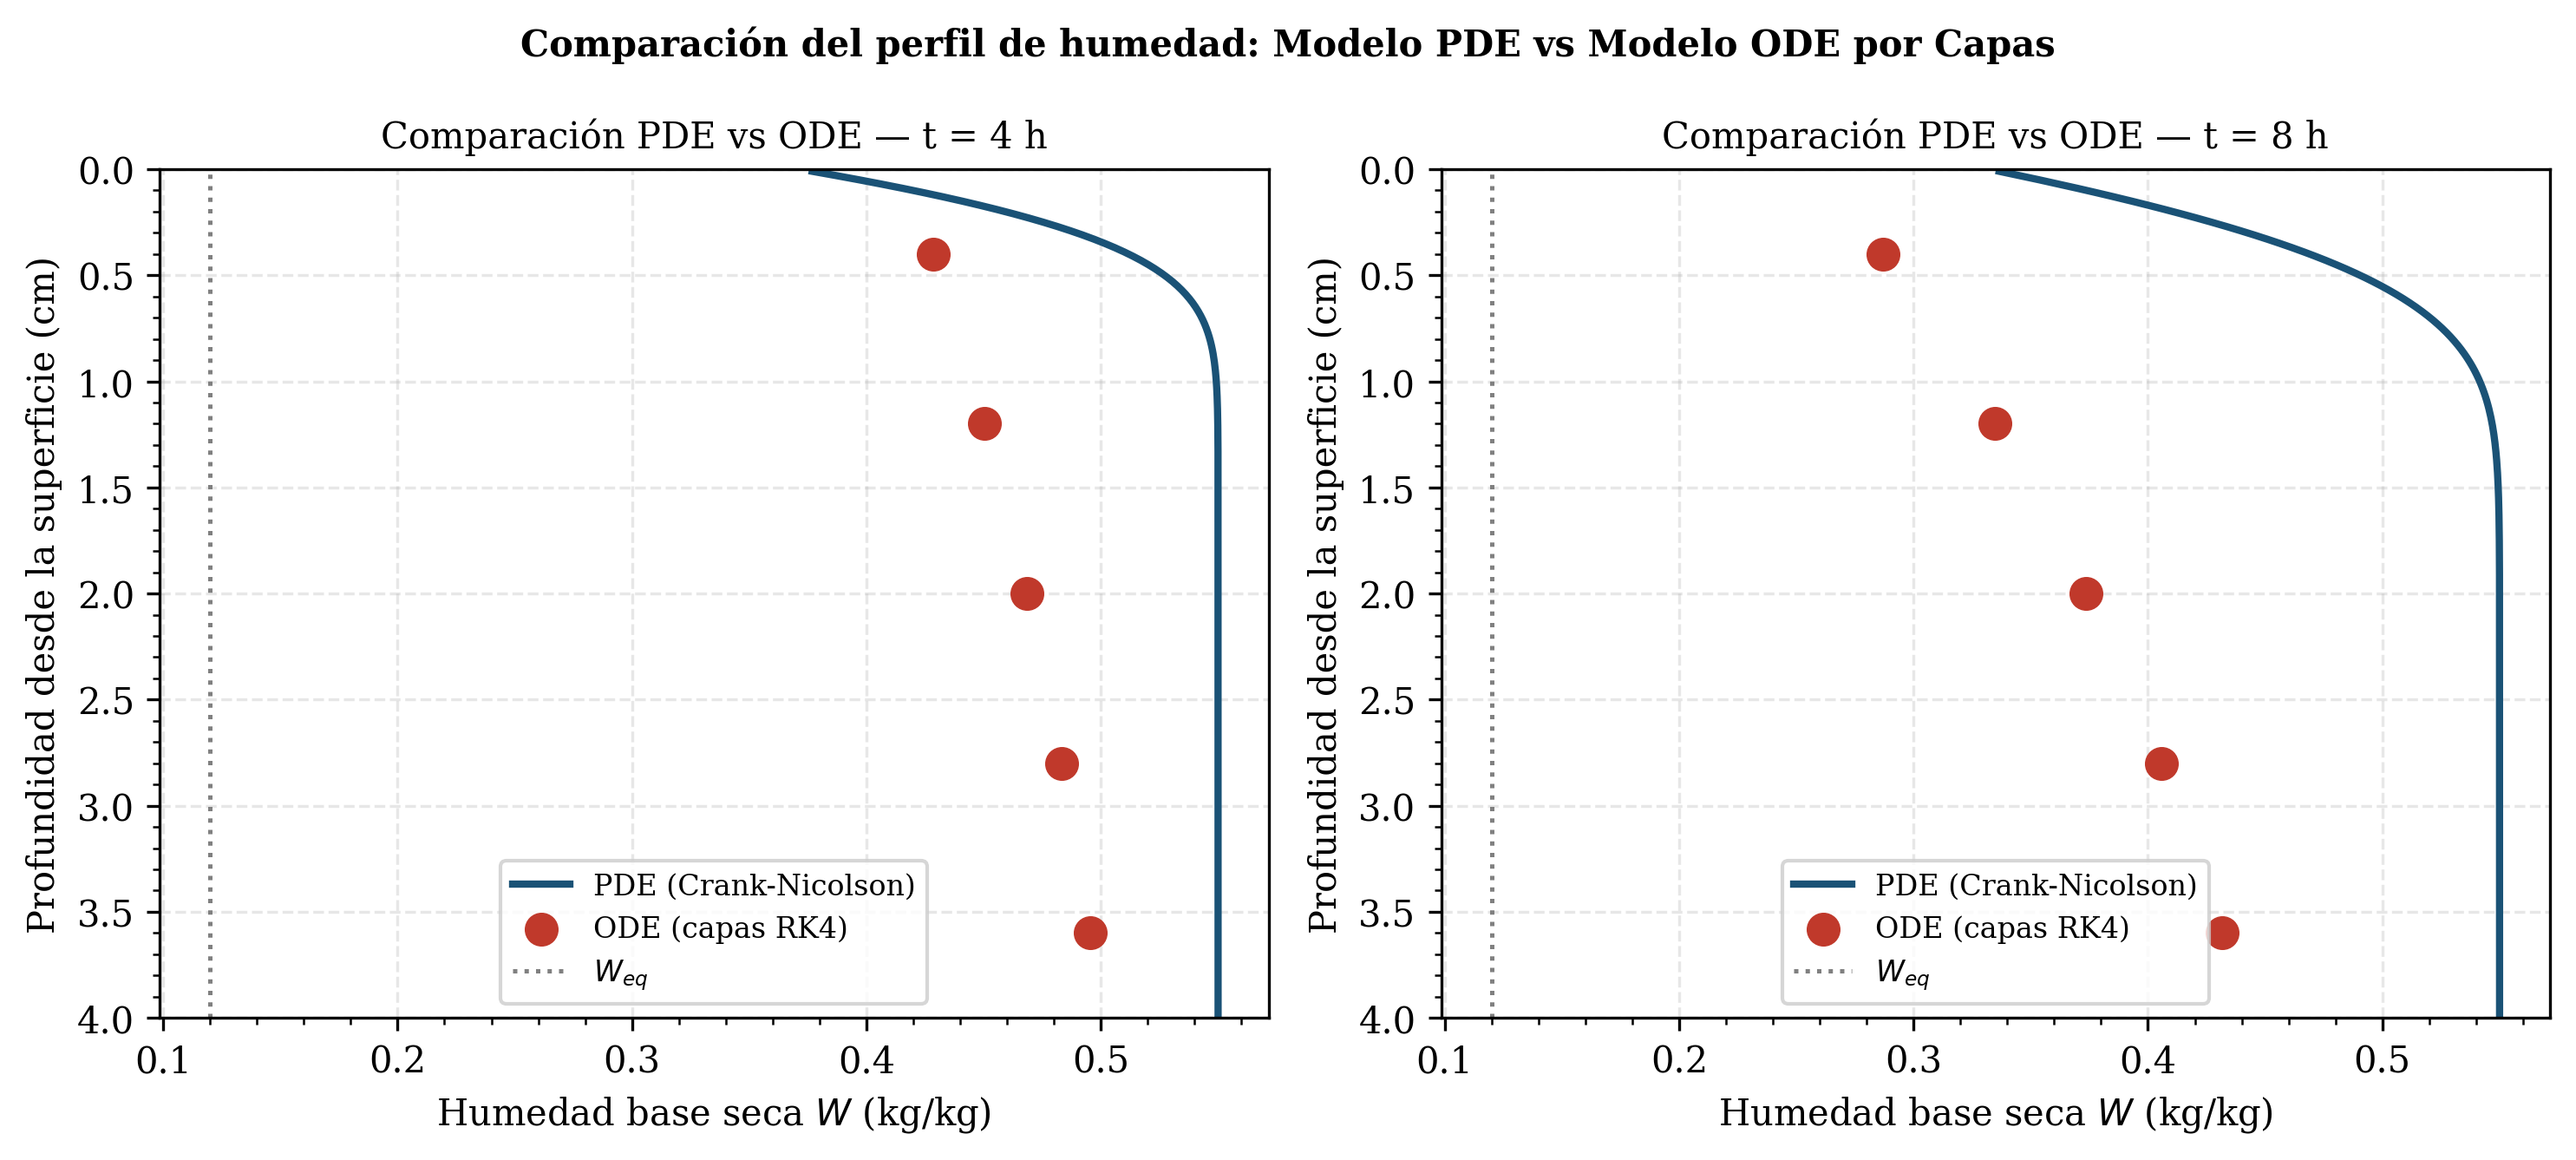
\includegraphics[width=0.48\textwidth]{pde_comparacion_ode.png}
\caption{Comparación del perfil de humedad entre el modelo PDE (Crank-Nicolson) y el modelo ODE por capas (RK4) a $t = 4\,\text{h}$ y $t = 8\,\text{h}$.}
\label{fig:pde_comparacion}
\end{figure}

\begin{table}[H]
\centering
\caption{Resultados del modelo PDE a $t = 8\,\text{h}$}
\begin{tabular}{lll}
\toprule
Variable & Valor & Unidad \\
\midrule
$W$ en superficie ($z=4\,\text{cm}$) & 0.337 & kg/kg (bs) \\
$W$ en centro      ($z=2\,\text{cm}$) & 0.550 & kg/kg (bs) \\
$W$ en fondo       ($z=0\,\text{cm}$) & 0.550 & kg/kg (bs) \\
Frente de secado $\delta$             & 0.76  & cm \\
Temperatura superficial               & 23.6  & °C \\
\bottomrule
\end{tabular}
\end{table}

\section{Conclusiones}

El modelo matemático desarrollado permitió representar adecuadamente el proceso de secado de café a dos escalas: el grano individual y la marquesina completa. La formulación mediante ecuaciones diferenciales ordinarias acopladas y su solución con el método RK4 produjeron resultados estables y físicamente coherentes.

La extensión del modelo a la marquesina mediante la formulación por capas con extinción exponencial captura el gradiente de humedad observado experimentalmente, donde la superficie de la cama se seca con mayor rapidez que las capas internas.

La simulación de la marquesina de 10~m~$\times$~4~m con aproximadamente 2.4~millones de granos mostró que, en condiciones climáticas andinas colombianas, se remueve alrededor del 33.4\% del agua inicial en 8~horas ($X_{bulk}$: 0.550 → 0.367~kg/kg~bs), siendo necesario extender el proceso durante varios días para alcanzar la humedad comercial de 11\% (base seca).

La herramienta computacional desarrollada constituye una base sólida para analizar el efecto de parámetros de diseño de la marquesina (dimensiones, profundidad de la cama, orientación) y para optimizar las condiciones de secado en finca.

\section{Referencias}

\begin{thebibliography}{99}

\bibitem{ref1}

K. N. Çerçi y M. Das,

``Modeling of heat transfer coefficient in solar greenhouse type drying systems,''

\textit{Sustainability},

vol. 11,
no. 19,
2019.

\bibitem{ref2}

H. J. Ciro-Velásquez et al.,

``Numerical simulation of thin layer coffee drying by control volumes,''

\textit{Dyna},

vol. 77,
2010.

\bibitem{ref3}

A. Parra-Coronado,
G. Roa-Mejía
y
C. E. Oliveros-Tascón,

``SECAFÉ Parte I: modelamiento y simulación matemática,''

\textit{Revista Brasileira de Engenharia Agrícola e Ambiental},

2008.

\end{thebibliography}

\end{document}